\documentclass[aps,physrev,reprint,superscriptaddress,amsmath,amssymb,floatfix]{revtex4-2}
% NOTE ON CLASS OPTIONS: revtex4-2 (v4.2f, dated 2022-06-05) does not ship a
% dedicated per-journal option for Physical Review Research -- there is no
% "prresearch" option in the distributed class. This was verified directly
% against the class's own source documentation (the journal-option list in
% revtex4-2.dtx enumerates prb, prc, prd, pre, prl, prper, prab, prx,
% prapplied, prmaterials, prfluids, physrev, and rmp; PRResearch is not
% among them). "physrev" is the class's documented generic/"future-proofing"
% option for APS Physical Review journals without their own dedicated style
% file, and is used here for exactly that reason. "reprint" gives the
% two-column, journal-approximating layout APS accepts for submission. See
% the accompanying summary document for how this was checked.

\usepackage{graphicx}
\usepackage{bm}
\usepackage{xcolor}
\usepackage{tikz}
\usetikzlibrary{arrows.meta,positioning,calc}
\definecolor{stablecol}{RGB}{31,97,141}
\definecolor{unstablecol}{RGB}{176,32,32}
\usepackage{placeins}
\usepackage{float}
% placeins gives \FloatBarrier, used below at each subsection boundary in
% Results/Discussion: with this many figures and tables competing for
% top-of-column space in revtex4-2's two-column "reprint" layout, LaTeX's
% default float algorithm lets figures drift many pages past the text that
% discusses them (observed up to ~8 pages). \FloatBarrier forces every
% figure/table introduced so far to be placed before the next section
% starts, keeping each figure visible near its own discussion.

\begin{document}

\title{Self-consistent electromagnetic feedback in Majorana nanowires:\\
a validated single-channel null result, and its breakdown beyond one subband}

\author{Arnav Rohilla}
\affiliation{Independent Researcher, Colorado, USA}
% NOTE: affiliation left as a placeholder for the user to
% complete -- see accompanying summary document.

\date{\today}

\begin{abstract}
Standard treatments of the Majorana nanowire fix the topological phase
boundary and compute the induced supercurrent afterward; the current is
never fed back into the Hamiltonian that produced it. We close this loop
with a validated framework -- a particle-hole-symmetric Bogoliubov-de
Gennes eigensolver, a real-space Pfaffian $\mathbb{Z}_2$ invariant, and a
Biot-Savart ring self-field -- so that the wire's self-generated flux
dresses the Peierls phase entering its own Hamiltonian. In the
single-channel limit this feedback produces no genuine bulk shift of the
topological boundary at any dynamically accessible coupling strength; the
null result is robust under finite-size scaling, ring-inductance
variation, operating temperature up to and beyond $20\,\mathrm{mK}$, and
on-site disorder at the lower end of a literature-grounded range. Two
results recur throughout: a conventional spectral-gap threshold detector
overstates the shift by an order of magnitude relative to the
threshold-free invariant, and the self-consistency loop has a dynamical
bifurcation above which a fixed point exists but is not
Picard-attracting, so existence and dynamical stability must be verified
independently. Extending the calculation to a second occupied transverse
subband overturns the null: a pre-registered loop-gain diagnostic crosses
the Picard stability threshold at the production electromagnetic
coupling once $M\geq2$, and a full self-consistent boundary calculation
at $M=2$ shows that the \emph{existence} of a static topological boundary
becomes fragile to the lattice discretization used to compute it.
Extending the same diagnostic to $M=5,6$ shows this trend is itself
non-monotonic, not a simple worsening with occupancy: the loop-gain
statistic collapses at $M=6$, but the underlying detachment rate --
whether any static solution exists at all -- stays high and
non-monotonic throughout, so existence, not the loop-gain magnitude,
remains the operative diagnostic. Because realistic InAs/Al devices are
estimated to occupy far more than two subbands, this existence-fragility
result -- not the single-channel null -- should govern how
electromagnetic feedback is treated in real devices. Code, validation
scripts, and raw data are publicly available.
\end{abstract}

\maketitle

\begin{figure*}[t]
\centering
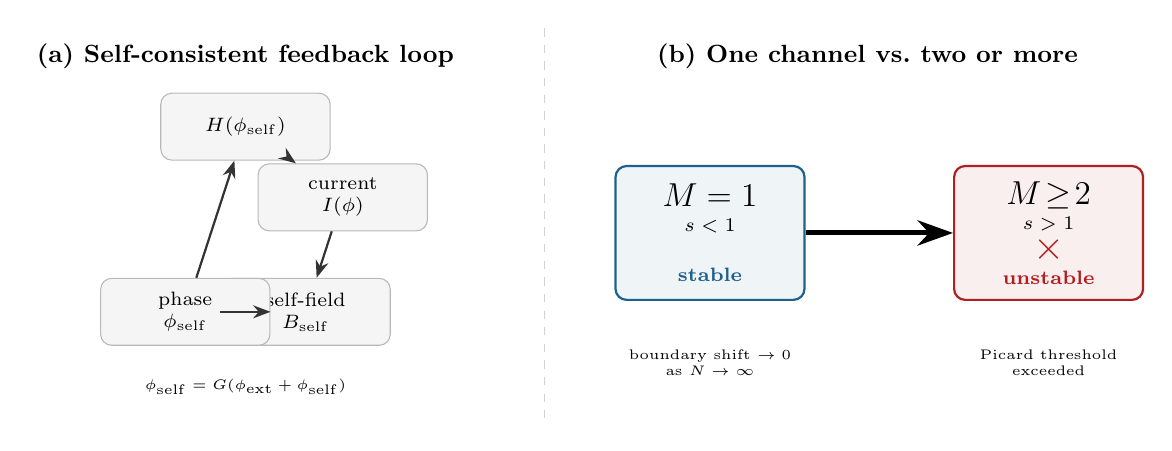
\begin{tikzpicture}[
  every node/.style={font=\small},
  proc/.style={draw, rounded corners, align=center, minimum width=2.15cm,
    minimum height=0.85cm, fill=gray!8, draw=gray!55, font=\scriptsize},
  panelttl/.style={font=\bfseries\small},
  outcome/.style={draw, thick, rounded corners, align=center,
    minimum width=2.4cm, minimum height=1.7cm, font=\scriptsize},
  loopar/.style={-{Stealth[length=2.2mm]}, thick, gray!40!black},
  bigar/.style={-{Stealth[length=4.5mm,width=3.2mm]}, line width=1.8pt, black},
]

\node[panelttl] at (-4.35,2.15) {(a) Self-consistent feedback loop};
\def\r{1.3cm}
\node[proc] (h1) at ($(-4.35,-0.05)+(90:\r)$)  {$H(\phi_{\rm self})$};
\node[proc] (h2) at ($(-4.35,-0.05)+(18:\r)$)  {current\\$I(\phi)$};
\node[proc] (h3) at ($(-4.35,-0.05)+(-54:\r)$) {self-field\\$B_{\rm self}$};
\node[proc] (h4) at ($(-4.35,-0.05)+(-126:\r)$){phase\\$\phi_{\rm self}$};
\draw[loopar] (h1) -- (h2);
\draw[loopar] (h2) -- (h3);
\draw[loopar] (h3) -- (h4);
\draw[loopar] (h4) -- (h1);
\node[font=\tiny] at (-4.35,-2.05) {$\phi_{\rm self}=G(\phi_{\rm ext}+\phi_{\rm self})$};

\draw[gray!35, dashed] (-0.55,2.5) -- (-0.55,-2.5);

\node[panelttl] at (3.55,2.15) {(b) One channel vs.\ two or more};
\node[outcome, draw=stablecol, fill=stablecol!7] (m1) at (1.55,-0.1)
  {\large $M=1$\\[1pt] {\scriptsize $s<1$}\\[1pt]
   \textcolor{stablecol}{\Large\checkmark}\\[1pt]
   \textcolor{stablecol}{\textbf{\scriptsize stable}}};
\node[outcome, draw=unstablecol, fill=unstablecol!7] (m2) at (5.85,-0.1)
  {\large $M\!\geq\!2$\\[1pt] {\scriptsize $s>1$}\\[1pt]
   \textcolor{unstablecol}{\Large$\times$}\\[1pt]
   \textcolor{unstablecol}{\textbf{\scriptsize unstable}}};
\draw[bigar] (m1) -- (m2);
\node[font=\tiny, align=center] at (1.55,-1.75) {boundary shift $\to0$\\as $N\to\infty$};
\node[font=\tiny, align=center] at (5.85,-1.75) {Picard threshold\\exceeded};
\end{tikzpicture}
\caption{\textbf{Graphical summary.} (a) The loop closed in this paper: a
bond-phase texture fixes $H$, whose ground-state current sources a
Biot-Savart self-field, whose Peierls phase feeds back into $H$. (b) The
central result: at $M=1$ the loop-gain slope stays sub-critical ($s<1$,
validated null); once a second transverse subband is occupied
($M\geq2$), $s$ crosses the Picard stability threshold at production
coupling and the static topological boundary itself becomes fragile.}
\label{fig:graphical_abstract}
\end{figure*}

\section{Introduction}
\label{sec:intro}

A one-dimensional topological superconductor supporting unpaired Majorana
zero modes (MZMs) at its ends was first shown by Kitaev to arise from a
spinless $p$-wave pairing model whose bulk topology is captured by a
$\mathbb{Z}_2$ invariant~\cite{kitaev2001}. Oreg, Refael, and von Oppen,
and independently Lutchyn, Sau, and Das Sarma, showed that the same
physics is realized in a much more accessible platform: a semiconducting
nanowire with strong Rashba spin-orbit coupling, placed in an external
Zeeman field and proximitized by an $s$-wave
superconductor~\cite{oreg2010,lutchyn2010}. This proposal launched over a
decade of experimental work on InAs/Al and InSb/Nb hybrid nanowires, whose
appeal for fault-tolerant quantum computation rests on the non-Abelian
exchange statistics of MZMs and the resulting topological protection of
information encoded in their collective fermion parity~\cite{lutchyn2018review}.

The experimental record is real but contested. Zero-bias conductance
peaks -- the original proposed signature -- have repeatedly been shown to
also arise from disorder-induced trivial Andreev bound states and other
non-topological mechanisms indistinguishable from a genuine Majorana
signature in tunneling conductance
alone~\cite{prada2020review,liu2018distinguishing}, and claims in this
field have a documented history of being revised or withdrawn under
closer scrutiny. Progress has continued: a 2025 measurement from Microsoft Quantum reported a
single-shot interferometric readout of fermion parity in an InAs-Al
hybrid device, with a reported assignment error of 1\%, framed explicitly
as a step toward -- not a demonstration of -- topological
qubits~\cite{aghaee2025}. That same measurement has since been the
subject of a direct methodological challenge: a comment by
Legg~\cite{legg2025} argues that the topological gap protocol used to
certify the device's gapped, disorder-free operating regime is
unreliable~\cite{legg2026nature} and that publicly available data in the
same regions used for the parity readout is, on direct inspection,
disordered with no clear gap. Microsoft Quantum has responded in a
formal reply~\cite{msreply2025}, which states that the objections are
unfounded and that no flaws have been identified in its estimate of the
protocol's false discovery rate, and the exchange has since appeared as a
comment and reply in \emph{Nature}~\cite{legg2026nature,msreply2026nature};
we take no position on its resolution. We report
this dispute as part of the field's current state, not as a resolved
matter either way. Distinguishing genuine topological physics from look-alike
trivial physics in a disordered, finite device remains the central open
problem in this field -- indeed, recent work argues that in short,
disordered wires the topological classification itself may not be
uniquely defined and requires context-dependent
analysis~\cite{pan2026} -- and it is the reason a validated,
threshold-free topological diagnostic -- not a spectral proxy -- is a
prerequisite for any claim made in this paper.

A second, largely separate line of question concerns the wire's
electromagnetic environment. Realistic Majorana device architectures
embed the nanowire in a circuit -- gate electrodes, coplanar-waveguide
resonators for dispersive readout, and the loop inductance of the
proximitizing superconductor itself. The current flowing in the wire, set
self-consistently by the wire's own quantum state, generates a magnetic
self-field; if that field is large enough, and slow enough on the
relevant timescale, it re-enters the Hamiltonian as a phase twist and
could in principle shift the very topological phase boundary the circuit
is built to read out. To our knowledge, no prior published work has
closed this loop for the electromagnetic (inductive, current-generated
flux) channel specifically together with a genuine, threshold-free
topological invariant. The closest related work addresses different
feedback channels or a different role for inductance entirely: Vuik
\emph{et al.}\ treat a self-consistent \emph{electrostatic} (Coulomb,
Schr\"odinger-Poisson) response of the chemical potential to an applied
field and show it reshapes the topological phase
boundary~\cite{vuik2016}; Lobo, Prada, and San-Jose treat a self-consistent
Hartree-Fock-Bogoliubov \emph{pairing potential} in intrinsic (non-hybrid)
wires~\cite{lobo2025}; Shustin, Aksenov, and Burmistrov compute
many-body \emph{charge-fluctuation} corrections to the topological
winding number via a Green's-function self-energy, distinct from any
classical electromagnetic self-field~\cite{shustin2024}; and Roy, Sau,
and Tewari propose quantum inductance as a phase-sensitive
\emph{diagnostic probe} of a fixed, non-self-consistent
Hamiltonian~\cite{roy2026inductance}, not as a mechanism that modifies the
boundary itself. Our work is the electromagnetic-feedback analogue of
Vuik \emph{et al.}'s electrostatic-feedback question, and we adopt the
same caution in framing it: the answer we find is a null result in the
regime we can fully validate, and a non-null, unresolved result beyond
it, not a clean confirmation in either direction.

We build and validate a computational framework that closes this loop
for a Lutchyn-Oreg nanowire on a ring geometry (\S\ref{sec:model}) and
report a findings arc organized around two axes: robustness of the
single-channel result, and its extension to a second occupied transverse
subband (\S\ref{sec:results}). The single-channel result is a validated
null: no bulk topological-boundary shift survives finite-size scaling,
variation of the wire's own inductance, realistic operating temperature,
or (at the lower end of the literature-realistic range) explicit on-site
disorder. Two methodological lessons recur throughout this arc and are
central to it: first, that a conventional
spectral-gap threshold detector is not a reliable proxy for the bulk
topological invariant, even at fixed system size, and produces an
order-of-magnitude-overstated boundary shift; second, that a
self-consistency loop of this kind possesses a genuine dynamical
bifurcation, above which mathematical fixed points continue to exist but
are no longer attracting under the physical relaxation dynamics -- so
existence and dynamical stability of a solution must always be checked as
two separate questions. Extending the calculation to two occupied
transverse subbands overturns this null result, and does so in a way that
is qualitatively more severe than a magnitude change: at the production
electromagnetic coupling, the loop gain crosses the stability threshold
once two or more subbands are occupied, and a full self-consistent
boundary calculation at a representative two-subband operating point
shows that the very existence of a static topological boundary becomes
fragile to the lattice discretization used to compute it. Given that
realistic InAs/Al devices are estimated to occupy far more than two
subbands~\cite{woods2020,chang2015}, we present this existence-fragility
result, not the single-channel null, as the paper's operative conclusion
for real devices (\S\ref{sec:discussion}).

Every result in this paper -- including intermediate results that were
later superseded by more rigorous checks -- is preserved and traceable in
a public code repository, together with every validation script and raw
output file; see the data availability statement at the end of this
paper.

\section{Model and computational framework}
\label{sec:model}

\subsection{Lutchyn-Oreg Hamiltonian and material parameters}

We use the standard real-space, tight-binding Lutchyn-Oreg BdG Hamiltonian
for a single conducting channel: a chain of $N$ sites with lattice
constant $a$, nearest-neighbor hopping $t$, Rashba spin-orbit coupling
$\alpha$, chemical potential $\mu$, in-plane Zeeman field $B$, and
$s$-wave proximity pairing $\Delta$, written in the Nambu basis
(electron/hole $\otimes$ spin $\otimes$ site, dimension $4N$) so that the
hole block is the exact conjugate of the electron block and
particle-hole (PH) symmetry $\Sigma_x H^* \Sigma_x = -H$ holds identically
for any parameter choice, including a spatially non-uniform phase
texture on the bonds. Energies are quoted in units of $\Delta$ unless
stated otherwise. Material parameters are drawn from InAs bulk properties
($m^*=0.023\,m_e$, $g$-factor $10.5$, $\alpha_{\rm SO}=20\;{\rm
meV\,nm}$)~\cite{oreg2010,lutchyn2010} and from the induced gap directly
measured in epitaxial-Al/InAs full-shell nanowires, $\Delta=0.19\;{\rm
meV}$~\cite{chang2015}, giving $t\approx 66.3\,\Delta$ and
$\alpha\approx8.0\,\Delta$ at $a=10\;{\rm nm}$. Chang \emph{et
al.}\ additionally report a base operating temperature of $20\;{\rm mK}$
and an axial critical field of $\approx75\;{\rm mT}$ for a comparable
thin epitaxial-Al shell~\cite{chang2015}; the latter is well below the
Zeeman field needed to reach this model's topological transition at
these parameters, so the model's own pairing potential $\Delta$ is held
fixed (no field-dependent pair-breaking $\Delta(B)$), an idealization we
carry explicitly through every figure and result that sweeps $B$ into
that regime.

\subsection{Topological invariant: a threshold-free real-space Pfaffian}

Rather than detecting the topological transition as the field at which
the lowest BdG excitation crosses a fixed absolute energy threshold, we
use the genuinely discrete $\mathbb{Z}_2$ invariant: the sign of the
Pfaffian of the Hamiltonian rotated into its Majorana (real
antisymmetric) basis~\cite{kitaev2001}. For a periodic ring we use the
periodic-boundary-condition (PBC) Pfaffian alone rather than the full
PBC$\times$antiperiodic-boundary-condition (APBC) product used in the
general real-space construction~\cite{pfaffian_realspace2026}: in this regime
the $k=\pi$ gap never closes near the transition and contributes only a
constant, non-flipping sign, while $k=0$ is an allowed ring momentum at
every system size $N$, so the boundary located this way carries
\emph{zero} measured finite-size shift, in contrast to the conventional
spectral threshold detector. We validate this construction against the
known analytic boundary at multiple chemical potentials, ring sizes, and
bisection tolerances, and against a threshold detector swept over its own
threshold at fixed $N$ (procedural detail in Appendix~\ref{app:gates};
outcomes summarized in the first three rows of Table~\ref{tab:gates}).
Results are given in \S\ref{subsec:threshold}.

A companion correction is recorded here as part of this framework's
validation discipline: an earlier module computing this same invariant
never actually called the Pfaffian routine it was supposed to, and the
bug survived undetected only because of a parameter regime in which a
hardcoded closed-form stand-in happened to agree with it. It was caught,
fixed, and re-validated with zero disagreements against the analytic
boundary across a $1600$-point sweep before any result relying on it was
trusted; full mechanism detail is recorded in the correction ledger
(Appendix~\ref{app:corrections}, item 2).

\subsection{Self-consistent electromagnetic feedback}

The physical motivation precedes the formalism. Once the Hamiltonian's
ground state is fixed at some applied field,
the wire carries a real, physical current circulating around the ring,
and that current is a genuine magnetic-field source. If the induced
self-field is large enough, and slow enough on the relevant electronic
timescale to be treated quasi-statically -- a separation of scales borne
out experimentally, since measured quasiparticle-poisoning (parity)
lifetimes in comparable proximitized hybrids reach the millisecond
range~\cite{higginbotham2015parity}, many orders of magnitude slower than
the induced gap's own $\hbar/\Delta\sim3.5\,\mathrm{ps}$ timescale at
$\Delta=0.19\;{\rm meV}$ -- it re-enters the same
additional phase on every hopping bond. This closes a feedback loop that
most prior treatments of this problem leave open, by computing the
induced current only after the topological phase boundary has already
been fixed and never feeding it back in.

\begin{figure}[t]
\centering
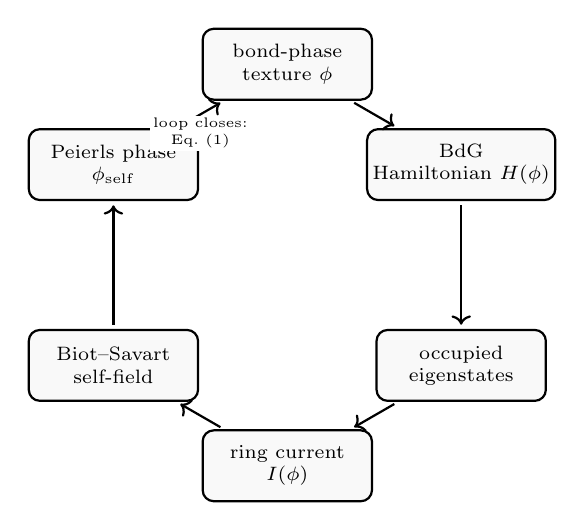
\begin{tikzpicture}[
  box/.style={draw, rounded corners, align=center, font=\scriptsize,
    minimum width=2.15cm, minimum height=0.9cm, fill=gray!5, inner sep=2pt},
  ->, thick, shorten >=1.5pt, shorten <=1.5pt
]
\def\r{2.55cm}
\node[box] (n1) at (90:\r)   {bond-phase\\texture $\phi$};
\node[box] (n2) at (30:\r)   {BdG\\Hamiltonian $H(\phi)$};
\node[box] (n3) at (-30:\r)  {occupied\\eigenstates};
\node[box] (n4) at (-90:\r)  {ring current\\$I(\phi)$};
\node[box] (n5) at (-150:\r) {Biot--Savart\\self-field};
\node[box] (n6) at (150:\r)  {Peierls phase\\$\phi_{\rm self}$};
\draw (n1) -- (n2);
\draw (n2) -- (n3);
\draw (n3) -- (n4);
\draw (n4) -- (n5);
\draw (n5) -- (n6);
\draw (n6) -- (n1) node[midway, below, font=\tiny, align=center, fill=white, inner sep=1pt]
  {loop closes:\\Eq.~(1)};
\end{tikzpicture}
\caption{\textbf{The feedback loop this paper closes: current sources
the very field that re-enters its own Hamiltonian.} Conceptual diagram,
not a data plot. A bond-phase texture fixes the BdG Hamiltonian, whose
occupied eigenstates carry a ring current; that current sources a
Biot-Savart self-field, which dresses the hopping bonds with an
additional Peierls phase that feeds back into the texture the loop
started from. The loop closes at the fixed-point condition of Eq.~(1),
$\phi_{\rm self}=G(\phi_{\rm ext}+\phi_{\rm self})$.}
\label{fig:loop}
\end{figure}

The wire is closed into a ring of circumference $L=Na$. The ring current
density $I(\phi)$, summed over occupied BdG quasiparticle states at a
given uniform bond-phase texture $\phi$, generates a magnetic self-field
via the Biot-Savart law adapted to the closed geometry (validated
against the analytic thin-wire loop self-inductance to better than
$0.5\%$), which re-enters the Hamiltonian as an additional Peierls phase
on every bond. The self-consistency condition is
\begin{equation}
\phi_{\rm self} = G(\phi_{\rm ext}+\phi_{\rm self}), \qquad
G(\phi) = g\,\frac{e}{\hbar}\,a\,A_{\rm self}\!\left[I(\phi)\right],
\end{equation}
where $g$ is a dimensionless effective electromagnetic feedback gain
representing the combined action of a resonant readout circuit (quality
factor $Q$) and the ratio of kinetic to geometric inductance in the
nanowire loop. Superconducting coplanar-waveguide resonators with
internal quality factors exceeding $10^6$--$10^7$ have been demonstrated
experimentally~\cite{megrant2012}, and nanowire loops with large
kinetic-inductance contributions relative to their bare geometric
inductance have likewise been realized~\cite{samkharadze2016}; combining
representative values from these two independent, literature-grounded
mechanisms motivates treating $g$ as a plausibility estimate spanning
several orders of magnitude around $g\sim10^4$--$10^6$, not a value
derived from a specific circuit design. We adopt $g_{\rm
production}=2.9\times10^4$ as the single coupling value used throughout
the production results below (\S\ref{sec:model}D), and separately
characterize the loop's behavior as a function of $g$ across this entire
plausibility range.

On a uniform ring the self-consistency condition reduces to a scalar
fixed-point equation in $\phi$. We solve it three independent ways: (i)
bisection on $G(\phi)-\phi=0$, which requires no stability property of
the map and locates a root regardless of whether ordinary iteration would
converge to it; (ii) plain (Picard) fixed-point iteration, which
converges only where the map's local slope $s\equiv
dG/d\phi|_{\phi^*}$ satisfies $|s|<1$; and (iii) Anderson-accelerated
mixing, a quasi-Newton method that can locate a root even where the bare
map is Picard-repelling, gated on both a step-size criterion and an
independent fixed-point-residual check so that a stalled iterate is never
mistaken for a converged one. A Newton-Krylov search over the full
$N$-dimensional (non-uniform) fixed-point equation is used to test
directly whether any symmetry-broken solution exists beyond the uniform
one (seeding protocol in Appendix~\ref{app:gates}). This
three(-plus-one)-solver redundancy is what let us distinguish, as
described in \S\ref{subsec:bifurcation}, a root's mathematical existence from
its dynamical attractiveness -- a distinction that turns out to matter
throughout this paper.

\FloatBarrier
\subsection{Multi-subband extension}

To go beyond a single conducting channel we extend the basis to
site$(N)\otimes$subband$(M)\otimes$spin$(2)\otimes$Nambu$(2)$, dimension
$4NM$ (not $4NM^2$): each subband contributes a diagonal $4N$ block at
its own shifted chemical potential $\mu-\varepsilon_n$, plus a
mandatory inter-subband Rashba coupling $\propto\langle n|k_y|m\rangle$
that vanishes for even $n-m$ and is otherwise fixed by the hard-wall
transverse mode overlap. Omitting this term would not be a mere
approximation: it is the mechanism by which multiband occupancy
hybridizes Majorana pairs from different transverse modes and closes the
effective gap~\cite{lim2012}, so a model that dropped it would be
qualitatively, not just quantitatively, wrong. The construction is
validated by four gates before any physics result is trusted: exact
reproduction of the single-channel Hamiltonian and current operator at
$M=1$; exact decoupled-limit agreement with the direct sum of $M$
single-channel blocks when the inter-subband coupling is set to zero;
particle-hole symmetry at machine precision for $M=1$--$4$; and an exact
match of the inter-subband coupling matrix to its closed-form selection
rule. All four gates pass exactly.

The construction fixes a transverse hard-wall width $W=50\,\mathrm{nm}$,
chosen together with the van Hove exclusion tolerance below so that the
exclusion radius stays a small fraction of one subband spacing at every
$M$ tested. This gives a first-subband energy $\varepsilon_1\approx26.2\,\Delta$
and a full subband spacing growing from $\Delta E_{\rm
sb}(1)\approx19.6\,\Delta$ to $\Delta E_{\rm sb}(6)\approx85.0\,\Delta$
across the range tested below -- large compared to the $\sim2$--$30\;{\rm
meV}$ (order a few to several tens of $\Delta$) inter-subband spacings
Woods \emph{et al.}\ report across their modeled gate-charge range for
InAs/Al devices~\cite{woods2020}. The present construction therefore
resolves each newly occupied channel cleanly from its neighbors, at the
cost of not matching any specific real device's cross-sectional
geometry -- a structural, not device-faithful, choice, consistent with
every other idealization carried through this study.

Because the loop-gain slope $s$ is expected on general grounds to be
structured near any subband threshold (a one-dimensional van Hove
singularity in the density of states) rather than smooth in the
chemical potential, we pre-register -- in a separate commit, before any
value of $s(\mu;M)$ is computed -- a van Hove exclusion radius derived in
closed form from the bare tight-binding dispersion (and verified against
a genuinely diagonalized spectrum at threshold, not merely the smooth
bulk), a $\mu$-sweep window for each subband count $M$ that straddles its
own occupation threshold, and a comparison statistic (the median of
$s(\mu)$ over the surviving, non-excluded window, chosen over the
maximum specifically because the maximum would be pulled toward whatever
point sits nearest an excluded boundary). This locked-before-outcome
protocol mirrors the discipline this project applied after an earlier,
unqualified coupling-strength headline turned out to describe a
dynamically unreachable root (\S\ref{subsec:bifurcation}): fix the analysis
before the number that could be affected by it exists.

\subsection{Disorder and finite temperature}

On-site disorder is added as $\varepsilon_i\sim{\rm
Uniform}[-W/2,W/2]$, i.i.d.\ over sites, which preserves the PH-symmetry
identity exactly for any realization (verified both algebraically and
numerically). Every reported disordered quantity is an ensemble average
over independent realizations drawn with an explicit, reproducible
multiprocessing-safe seeding scheme, with the realization count and its
spread reported alongside every mean. The realistic disorder strength is
grounded directly in a re-verified primary source: Ahn \emph{et al.}\
report an on-site random potential with standard deviation
$\sigma_\mu=2.5\;{\rm meV}$ for InAs/InSb Majorana
nanowires~\cite{ahn2021}, which converts (with the conversion factor
itself flagged as the softest number in this part of the calculation,
since it depends on matching a Gaussian literature disorder model to this
work's uniform-distribution convention) to $W\approx10$--$46\,\Delta$ at
our $\Delta$.

Finite temperature enters through Fermi-Dirac occupation of the BdG
quasiparticle spectrum, applied to the self-field current, the boundary
detector, and a finite-frequency current-current (Kubo) correlator used
for the reactive-impedance diagnostic below; every finite-temperature
quantity is validated to reproduce its zero-temperature counterpart
bit-for-bit (or, for the Kubo correlator, to floating-point precision) as
$\theta\equiv k_BT/\Delta\to0$.

\subsection{Reactive impedance diagnostic}

As a second, independent observable alongside the bulk gap, we define a
feedback-renormalized reactance $Z_r(\omega)=i\omega L_{\rm eff}$,
$L_{\rm eff}=L_{\rm geo}/(1-s)$, where $s$ is the same self-consistency
loop-gain slope defined above and $L_{\rm geo}$ is the geometric
self-inductance of the ring, independently validated against the
analytic thin-wire loop formula. This linearization of the closed-loop
response diverges precisely at the Picard bifurcation $s\to1$, giving a
circuit-level observable sensitive to the same instability the
self-consistency solver encounters directly. We cross-check its
zero-frequency limit against a finite-frequency Kubo current-current
correlator computed from the full BdG spectrum (a fully independent,
non-reused calculation), which must reduce to $L_{\rm eff}$ as
$\omega\to0$; this cross-check is a required gate, not a reported result,
and failing it would indicate a bug rather than new physics.

\subsection{Data availability}
\label{sec:dataavail}
The complete codebase used to produce every result in this paper --
including every validation script referenced above, all raw numerical
results (as JSON/CSV data files), and every figure-generating script --
is publicly available in the GitHub repository
\texttt{majorana-nanowire-em-feedback} accompanying this work
(\url{https://github.com/MidnightNotHere/majorana-nanowire-em-feedback}).
Superseded intermediate results (see, e.g., \S\ref{subsec:robustness} and \S\ref{subsec:proxy})
are preserved in the repository rather than overwritten, with the
correction and its reasoning recorded alongside.

\FloatBarrier
\section{Results}
\label{sec:results}

\subsection{A conventional threshold detector overstates the boundary shift by an order of magnitude}
\label{subsec:threshold}

\begin{figure}[t]
\centering
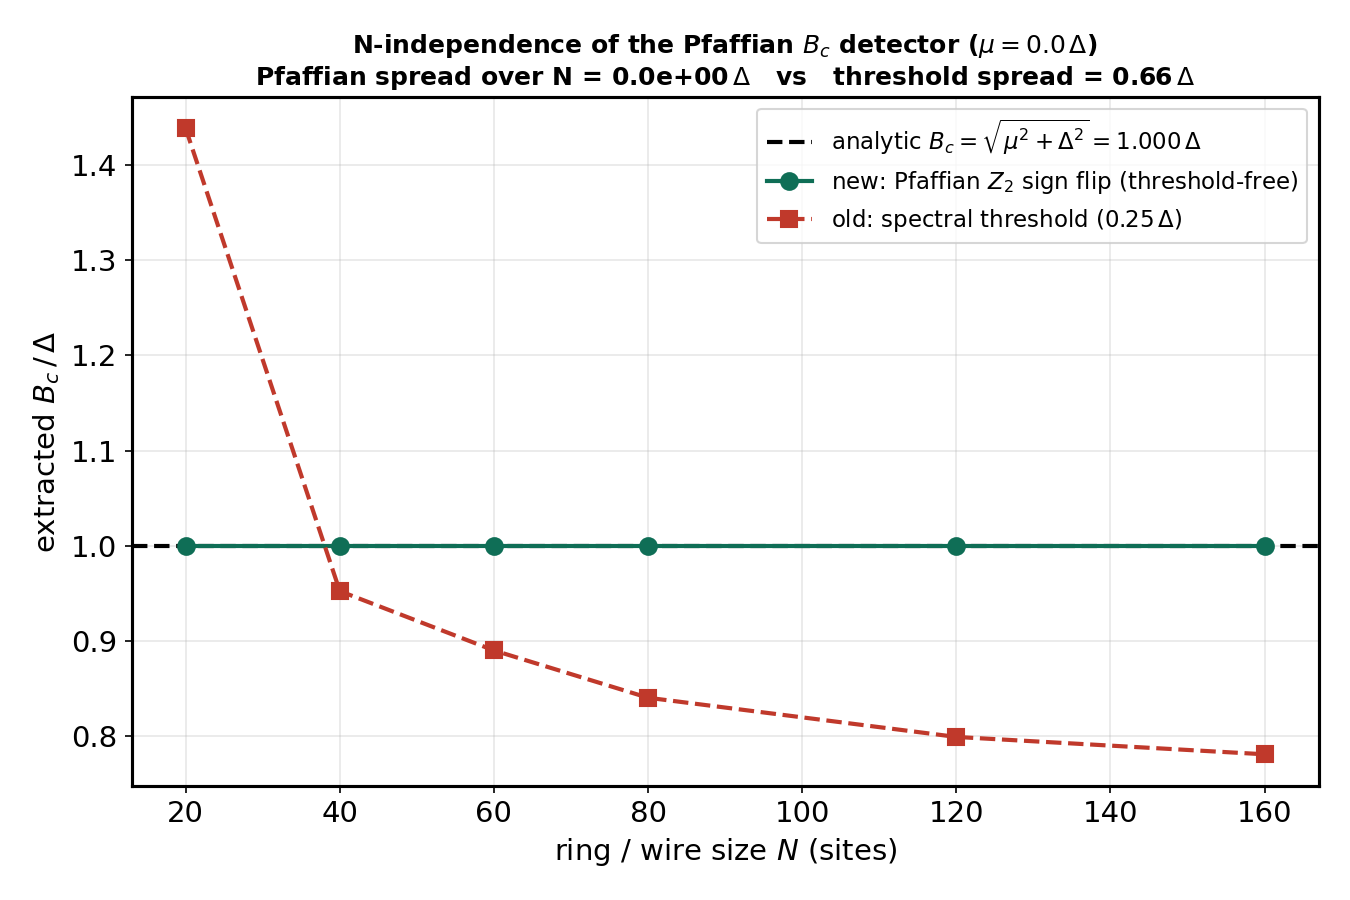
\includegraphics[width=\columnwidth]{figures/fig2_pfaffian_vs_threshold.png}
\caption{\textbf{The threshold-free Pfaffian invariant is exactly
$N$-independent; the conventional spectral-gap threshold detector is
not.} $N$-independence of the real-space Pfaffian boundary detector
versus a conventional spectral-gap threshold detector, at $\mu=0$ (known
analytic boundary $B_c=\Delta$). The Pfaffian detector's extracted $B_c$
is exactly $N$-independent (spread $0.0$ across $N=20$--$160$); the
threshold detector's extracted $B_c$ drifts by $0.66\,\Delta$ over the
same range -- the concrete numerical origin of the order-of-magnitude
boundary-shift discrepancy reported in the text. Generated by
\texttt{bdg\_r4\_em\_coupling.py}; the figure is saved in \texttt{results/em\_\allowbreak feedback\_\allowbreak detector\_\allowbreak comparison/} (this module saves no data file).}
\label{fig:threshold}
\end{figure}

Intuitively, the two detectors are asking different kinds of questions
in the first place. A spectral-gap threshold detector asks whether the
lowest excitation energy has dropped below some chosen cutoff -- a
question about a \emph{magnitude}, which has no way to distinguish a
genuine bulk gap closing from an ordinary, non-topological state that
simply happens to sit below that same cutoff. A Pfaffian invariant asks a
fundamentally different, discrete question -- the \emph{sign} of a
Pfaffian, which can only change at a genuine gap closing -- so it cannot
be ``fooled'' by a state that is merely small. This distinction is not
just conceptual; it has a concrete, measured consequence below.

A spectral-gap threshold detector -- flagging the topological transition
as the field at which the lowest BdG excitation first drops below a
fixed fraction of $\Delta$ -- is sensitive to ordinary, non-topological
finite-size sub-gap structure whose level spacing shrinks with system
size, in a way that biases the detected boundary in the \emph{same}
direction growing $N$ would be expected to \emph{improve} a genuine
transition. Sweeping the threshold at fixed $N=80,\mu=0$ moves the
reported boundary across a $\sim$50-percentage-point band (from $+17.1\%$
at threshold $0.05\,\Delta$ to $-33.5\%$ at threshold $0.40\,\Delta$
relative to the analytic value); the reported offset also grows with $N$
in the wrong direction for a genuine (exponentially size-suppressed)
Majorana hybridization effect. The real-space Pfaffian invariant used
throughout this paper does not suffer from this: as
Fig.~\ref{fig:threshold} shows, its extracted boundary is exactly
$N$-independent across $N=20$--$160$ at $\mu=0$, and, checked separately
at the operating chemical potential and at two non-round values of
$\mu$, agrees with the analytic boundary to within bisection tolerance
at every system size tested.

The consequence for the actual boundary-shift headline is not merely
cosmetic. Holding the identical self-field texture fixed and swapping
only the detector, the threshold detector reports a shift of $-5.86\%$
($\mu=1.2$) and $-9.36\%$ ($\mu=1.4$), while the Pfaffian detector reports
$-0.77\%$ and $-0.60\%$ at the same two points -- roughly an order of
magnitude smaller, with the ranking between the two $\mu$ values reversed.
The sign (topological region marginally expanding under this particular,
not-yet-self-consistent self-field) survives; the magnitude reported by
the conventional detector does not. Every headline number quoted below
uses the Pfaffian detector exclusively.

\FloatBarrier
\subsection{The self-consistency loop has a genuine dynamical bifurcation}
\label{subsec:bifurcation}

\begin{figure}[t]
\centering
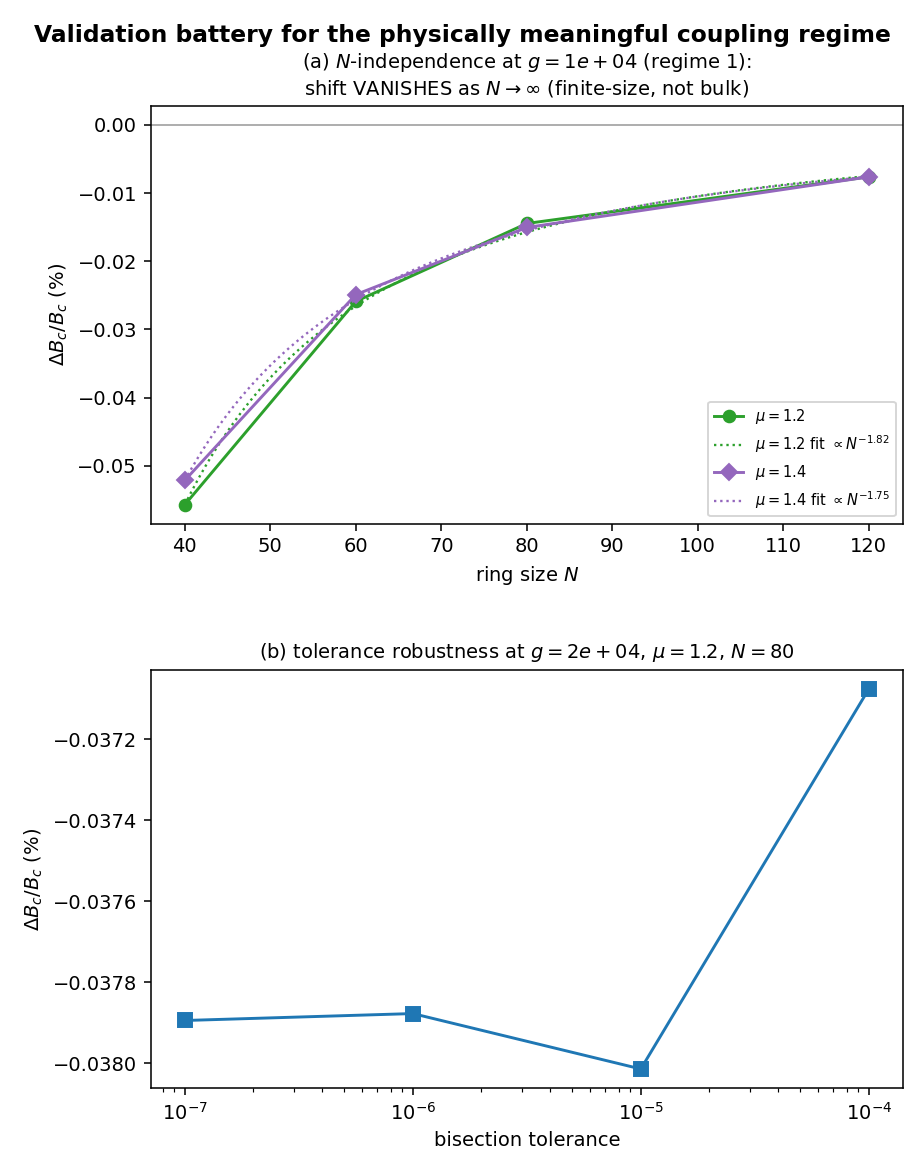
\includegraphics[width=\columnwidth]{figures/fig3_null_validation.png}
\caption{\textbf{The single-channel boundary shift vanishes as
$N\to\infty$: a finite-size artifact, not a genuine bulk effect.}
Validation battery for the physically meaningful coupling regime
($g<g_{\rm deadzone}$, top of the unambiguous static-boundary regime).
(a) $N$-independence of the boundary shift at $g=1\times10^4$: the shift
decays smoothly to zero as $N\to\infty$ ($\sim N^{-1.8}$ to $N^{-1.9}$),
the signature of a boundary (Aharonov-Bohm-like) effect rather than a
bulk one. (b) Bisection-tolerance robustness at $g=2\times10^4$, $N=80$:
the same shift is stable across four orders of magnitude of numerical
precision, ruling out a solver-tolerance artifact. Generated by
\texttt{scripts/\allowbreak redraw\_\allowbreak paper\_\allowbreak fig3.\allowbreak py} from
\texttt{results/\allowbreak self\_\allowbreak consistency\_\allowbreak bifurcation/\allowbreak r5\_\allowbreak physical\_\allowbreak shift\_\allowbreak results.\allowbreak json}, which
\texttt{bdg\_\allowbreak r5\_\allowbreak physically\_\allowbreak meaningful\_\allowbreak shift.\allowbreak py} writes.}
\label{fig:nullvalidation}
\end{figure}

Making the ring self-field genuinely self-consistent (rather than seeded
from an open-wire texture) at an initially assumed coupling
$g_0=3\times10^5$ produces a well-defined, gauge-checked, finite-size-
scaling-checked boundary shift of $+0.05\%$ at $N=80$. Taken at face
value this appears to be a small, validated, physical result. It is not:
plain Picard iteration does not converge at $g_0$ from any tested seed,
because the scalar self-consistency map's local slope there is $s\approx
3>1$ -- the fixed point found by bisection is a genuine mathematical root
of the self-consistency equation, but it is Picard-\emph{repelling}. A
direct scan of the map's slope across the coupling range establishes a
critical coupling $g_{\rm crit}\approx1.1$--$1.2\times10^5$: below it the
static boundary is unambiguous everywhere across the transition; in a
narrow intermediate band a dead-zone (no fixed point at all, not a
repelling one) opens exactly at the gap-closing field, where the
self-consistency map's characteristic sawtooth structure jumps across the
identity line without crossing it; above it, no attracting fixed point
exists anywhere near the transition, and $g_0=3\times10^5$ lies in this
regime. The mathematically valid $+0.05\%$ root is therefore a
dynamically unreachable solution, not a static equilibrium a real,
relaxing wire-circuit system would settle into.

Restricting the reported shift to the unambiguous regime ($g\lesssim
2.9\times10^4$, the value we subsequently adopt as $g_{\rm production}$)
gives a small, \emph{negative}, monotonically $g$-dependent,
path-independent shift that vanishes as $g\to0$ (as it must on physical
grounds): $\Delta B_c/B_c\approx-0.064\%$ ($\mu=1.2$) and $-0.066\%$
($\mu=1.4$) at $N=80$. Figure~\ref{fig:nullvalidation} shows the decisive
test: at fixed $g$, this shift vanishes as $N\to\infty$
($\sim N^{-1.8}$ to $N^{-1.9}$), and is robust under four orders of
magnitude of bisection-tolerance refinement. It is, in other words, a
finite-size Aharonov-Bohm flux artifact, not a genuine bulk effect.
Physically, this is what one would expect from a boundary phenomenon
rather than a bulk one: the self-consistent loop pins a roughly fixed
total self-flux threading the ring, so the quantity that actually enters
the Hamiltonian and could move the boundary -- the self-phase per lattice
bond -- is that fixed flux diluted over $N$ bonds, in the same way
persistent-current and flux-quantization effects in finite normal-metal
or superconducting rings are boundary phenomena that shrink as the ring
grows and vanish in the thermodynamic limit. A genuine bulk effect would
not be expected to shrink simply because the same physical system is
discretized more finely, which is exactly the property the $N$-independence
scans throughout this paper are designed to test.

Anderson-accelerated mixing independently confirms the picture above
rather than overturning it: it \emph{does} converge above $g_{\rm crit}$,
reaching the identical root the bisection solver finds (to six digits),
$\sim20\times$ faster, and reproducing the same finite-size scaling
$(\sim N^{-1.5})$ to zero in the bulk. What Anderson mixing changes is
only the precise statement of what $g_{\rm crit}$ means: it is a
threshold for the \emph{stability of a specific (Picard) iteration
scheme}, not a barrier to locating the mathematical equilibrium itself --
a real analog feedback circuit relaxing toward equilibrium implements
(approximately) Picard dynamics, so the physical instability above
$g_{\rm crit}$ stands even though a quasi-Newton solver can still find the
root. This root-existence-versus-dynamical-attractiveness distinction,
first established here, recurs as the operative lens for every non-null
result later in this paper (\S\ref{subsec:proxy},~\ref{subsec:existence}).

Separately varying the ring's circumference (hence its geometric
inductance) as a third axis, at fixed production coupling, shows that the
circuit inductance itself does not produce a bulk shift: where a static
boundary is well defined ($L\gtrsim0.8\,\mu$m), the shift is again tiny
($<0.07\%$) and vanishes under mesh refinement at \emph{fixed} physical
length ($\sim N^{-3.1}$, even faster than the fixed-lattice-constant
scaling above, since the self-field feedback is set by the per-bond
phase $\propto a=L/N$). The only genuinely length-dependent effect found
is not a bulk shift but a dynamical-stability threshold: sufficiently
short wires ($L\lesssim0.6\,\mu$m) lose the clean static boundary
entirely at this coupling, falling into the dead-zone regime described
above.

\FloatBarrier
\subsection{A second observable: the feedback-renormalized reactance}
\label{subsec:impedance}

The topological gap is not the only quantity the feedback loop dresses.
Because the self-consistent bond phase is proportional to magnetic flux,
and flux to inductance, linearizing the closed loop renormalizes the
ring's bare geometric inductance to $L_{\rm eff}=L_{\rm geo}/(1-s)$, where
$s\equiv dG/d\phi|_{\phi^*}$ is the loop-gain slope at the fixed point.
This defines a circuit-level reactive observable, $Z_r=i\omega L_{\rm
eff}$, which diverges as $s\to1$ and is therefore in principle sensitive to
physics the $g$-independent bulk gap cannot see. We compute it three ways
-- a static feedback-renormalized reactance, a finite-frequency Kubo
current-current correlator, and a variant whose source current includes
the spin-orbit contribution self-consistently -- and require, as a
validation gate, that the zero-frequency limit of the Kubo calculation
reproduce the static one; it does, to a relative mismatch of order
$10^{-4}$ at every clean grid point, holding even in the near-degenerate
region approaching the boundary.

\begin{figure}[t]
\centering
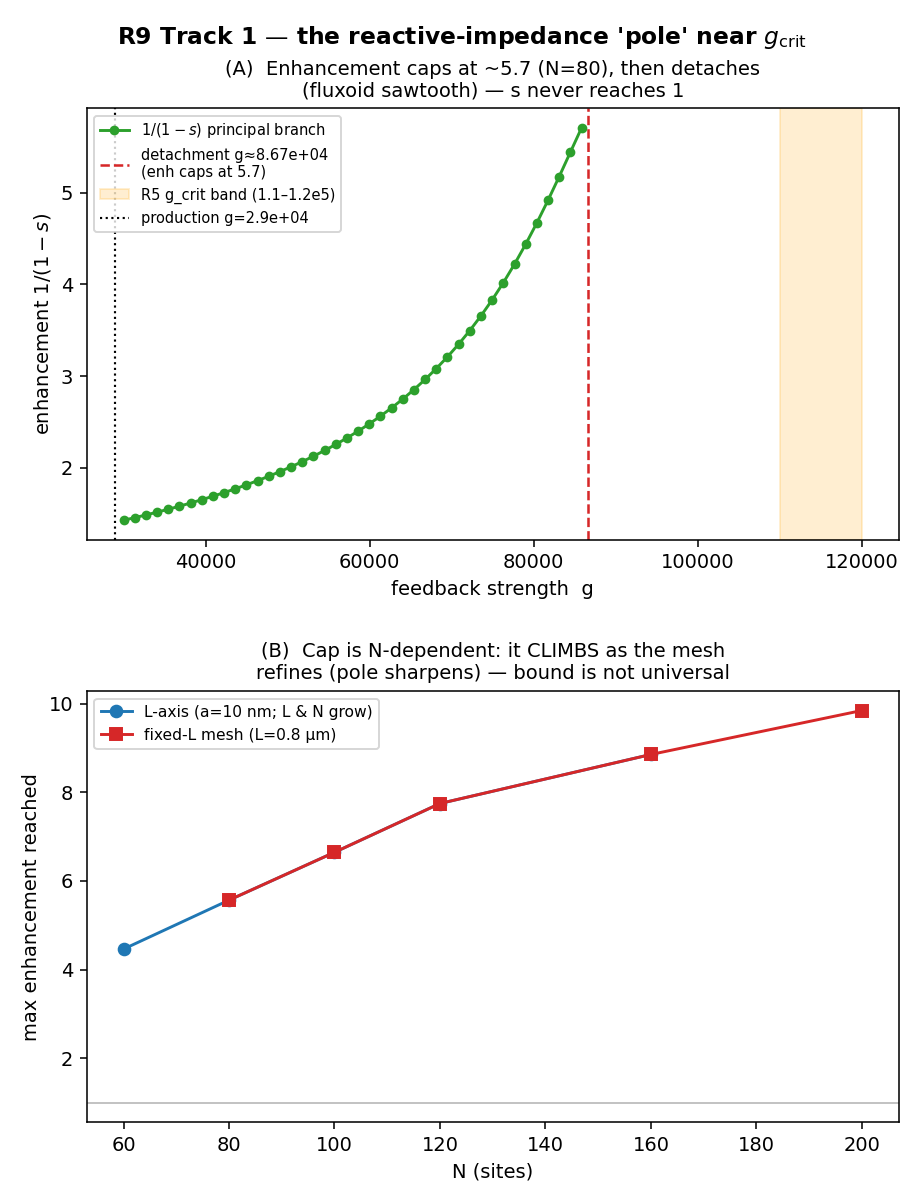
\includegraphics[width=\columnwidth]{figures/fig4_bounded_pole.png}
\caption{\textbf{The reactive-impedance enhancement saturates at a
bounded maximum instead of diverging.} The enhancement $1/(1-s)$ near
$g_{\rm crit}$. (A) On the physical principal branch the enhancement
rises smoothly to a bounded maximum ($\sim5.7\times$ at $N=80$) before
the static fixed point detaches via the self-consistency map's sawtooth
structure -- a literal $s=1$ divergence is never reached. (B) The bounded
cap itself is resolution-sensitive: it grows under mesh refinement at
fixed physical length ($\sim5.6\times$ at $N=80$ to $\sim9.8\times$ at
$N=200$), so a genuine continuum divergence is neither established nor
excluded by this data. Generated by
\texttt{scripts/\allowbreak redraw\_\allowbreak paper\_\allowbreak fig4.\allowbreak py} from
\texttt{results/\allowbreak reactive\_\allowbreak impedance/\allowbreak pole\_\allowbreak characterization/\allowbreak r9\_\allowbreak pole\_\allowbreak data.\allowbreak json}, which
\texttt{bdg\_\allowbreak r9\_\allowbreak pole\_\allowbreak characterization.\allowbreak py} writes.}
\label{fig:pole}
\end{figure}

Its one candidate orthogonal feature -- an apparent divergence of the
enhancement $1/(1-s)$ as $s\to1$ -- turns out, on direct characterization
with a root-finder immune to iteration instability, not to be a realized
divergence at all (Fig.~\ref{fig:pole}). On the physical principal branch
the enhancement rises smoothly to a \emph{bounded} maximum ($\sim5.7\times$
at $N=80$, where $s$ plateaus at $\approx0.825$) before the static fixed
point detaches via the same sawtooth mechanism identified in
\S\ref{subsec:bifurcation}, at $g\approx8.67\times10^4$ -- the leading edge
of that same bifurcation, reached here from the reactive-impedance side.
Physically, $1/(1-s)$ is exactly the factor by which feedback renormalizes
the ring's effective inductance above its bare geometric value,
$L_{\rm eff}=L_{\rm geo}/(1-s)$: as $s$ climbs toward its plateau the
circuit increasingly ``looks'' more inductive than its geometry alone
would suggest, and the point where the fixed point detaches is not a
separate phenomenon but the reactive-impedance signature of the same
underlying self-consistent state ceasing to be well-defined -- the
renormalization is capped exactly where the loop it depends on runs out
of an equilibrium to renormalize around. The cap is not universal: it grows under mesh refinement at fixed physical
length (from $\sim5.6\times$ at $N=80$ to $\sim9.8\times$ at $N=200$), so a
genuine continuum divergence is neither demonstrated nor excluded. The
finite-frequency calculation further confirms the feature is purely
reactive -- no companion feature appears in the dissipative channel, and
the dissipation onset that does exist is a bulk-pairing feature that does
\emph{not} track the topological minigap -- and making the spin-orbit
source current self-consistent shifts $L_{\rm eff}$ by only a few percent,
itself a finite-size effect that vanishes under mesh refinement.

The verdict is that $Z_r$ carries essentially no topological information
the bulk gap does not: across the production coupling range it tracks the
gap, and its lone orthogonal feature is a soft, bounded,
resolution-sensitive marker of proximity to the dynamical instability of
\S\ref{subsec:bifurcation} -- informative qualitatively, but not a sharp
new diagnostic.

\FloatBarrier
\subsection{Robustness of the single-channel null to temperature and disorder}
\label{subsec:robustness}

At the realistic operating temperature of $20\;{\rm mK}$
($\theta\equiv k_BT/\Delta\approx0.009$, corresponding to a thermal
quasiparticle population of order $10^{-48}$ at the gap edge), every
result above is unchanged to well within its own finite-size uncertainty:
the boundary shift at $N=80$ is $-0.131\%$ versus $-0.132\%$ at exactly
$T=0$, and still decays as $\sim N^{-1.9}$ toward zero at every
temperature tested. Thermal effects only become numerically noticeable
far above this operating point ($\theta\gtrsim0.05$, $\approx110\;{\rm
mK}$, itself approaching this fixed-$\Delta$ model's validity ceiling),
where the boundary shift weakens further (more null, not less), and where
two genuinely new, $T=0$-absent features appear in the finite-frequency
dissipation spectrum: an intraband Drude peak and sub-gap absorption from
thermally excited quasiparticles. Both are undetectable at the realistic
operating point.

\begin{figure}[t]
\centering
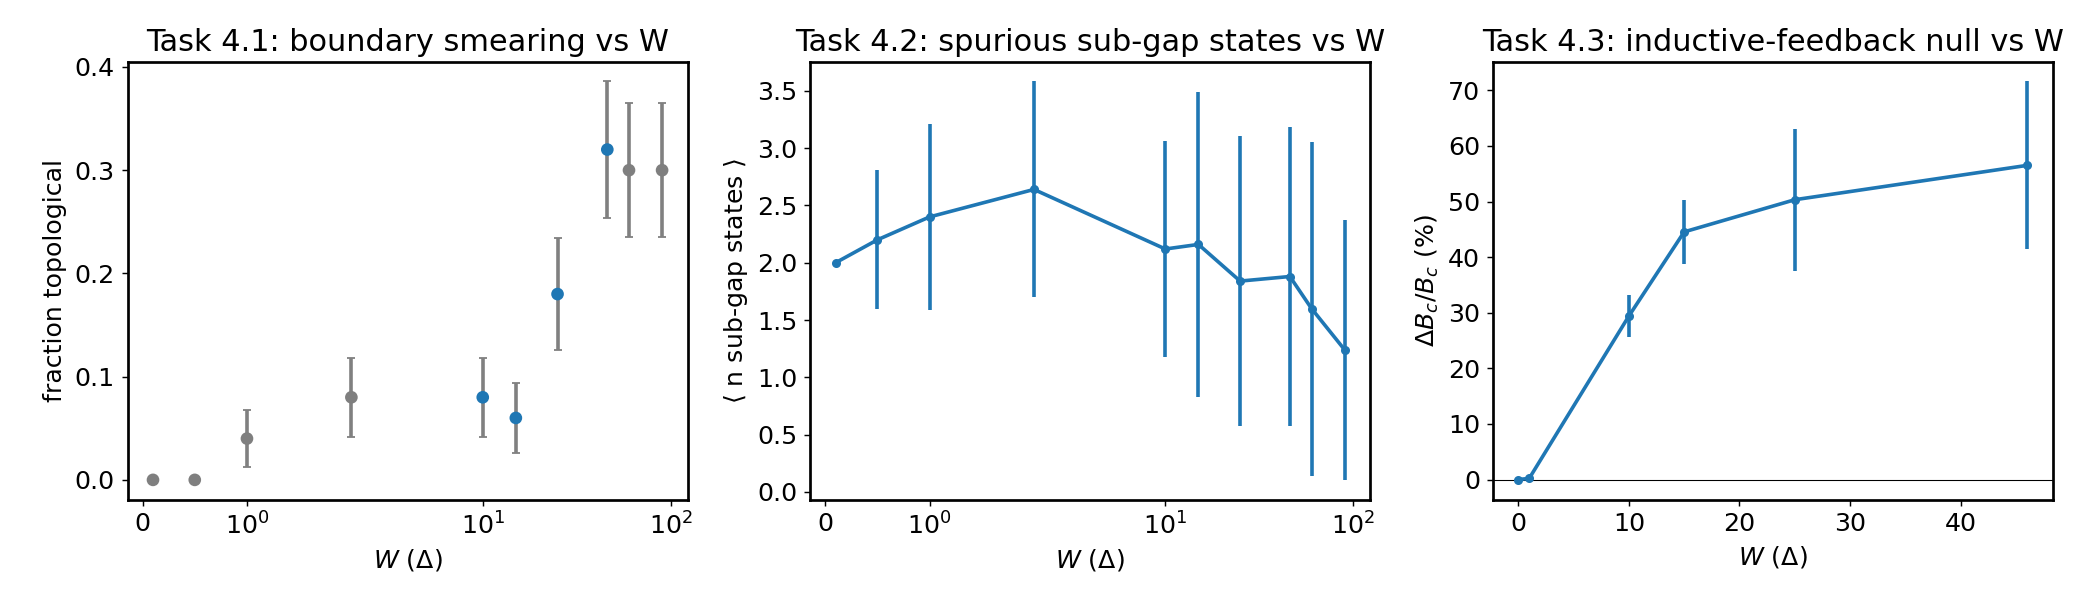
\includegraphics[width=\columnwidth]{figures/fig5_disorder_summary.png}
\caption{\textbf{Disorder smears the topological classification smoothly
and, at $N=80$ alone, appears to shift the self-consistent boundary --
an appearance later shown not to survive finite-size scrutiny at high
$W$.} On-site disorder at $N=80$: (left) fraction of realizations
misclassified as topological near a clean-trivial point, growing smoothly
and saturating near $30\%$ at the top of the literature-realistic range;
(middle) mean spurious sub-gap-state count (flat with $W$) versus its
realization-to-realization spread (growing substantially with $W$);
(right) mean self-consistent boundary shift versus $W$ at $N=80$ only.
\emph{The right-hand panel predates the finite-size scrutiny described in
the text}: a subsequent check at $N=120$ and $N=160$ found the $N=80$
values shown here substantially overstate the effect at the upper end of
the disorder range (\S\ref{subsec:robustness}) -- see
Table~\ref{tab:disorderNindep} for the corrected, size-scanned values.
Generated by \texttt{bdg\_r9\_disorder.py}; data in \texttt{results/disorder/}; the figure can be redrawn from the saved data with \texttt{scripts/\allowbreak redraw\_\allowbreak r9\_\allowbreak disorder\_\allowbreak summary.py}.}
\label{fig:disorder}
\end{figure}

\begin{table}[t]
\caption{Ensemble-averaged self-consistent boundary shift under on-site
disorder, at two points bracketing the literature-realistic range, as a
function of system size $N$ ($n_{\rm real}=30$ per point). The $N=80$
values are the same ones plotted in Fig.~\ref{fig:disorder}(right); they
substantially overstate the effect at $W=46\,\Delta$, which does not
survive to statistical significance once $N$ is increased.}
\label{tab:disorderNindep}
\begin{ruledtabular}
\begin{tabular}{cccc}
$N$ & shift, $W=10\,\Delta$ & shift, $W=46\,\Delta$ & $\sigma$ from 0 ($W=46\,\Delta$)\\
\hline
80  & $+29.4\%\pm3.8\%$  & $+56.5\%\pm15.1\%$ & $3.74$ \\
120 & $+19.8\%\pm3.4\%$  & $+9.6\%\pm8.2\%$   & $1.16$ \\
160 & $+22.6\%\pm3.7\%$  & $+10.8\%\pm7.2\%$  & $1.50$ \\
\end{tabular}
\end{ruledtabular}
\end{table}

On-site disorder is the one channel in the single-conducting-channel
study where the null result does not hold uniformly. Disorder measurably
and smoothly smears the topological boundary classification itself:
Fig.~\ref{fig:disorder}(left) shows the fraction of disorder realizations
misclassified as topological, at a point on the clean-trivial side of the
boundary, climbing through the literature-realistic disorder band and
saturating near $30\%$ at its upper end. The mean number of spurious
sub-gap states does not grow with disorder strength, but its
realization-to-realization spread does, growing from zero at weak
disorder to a magnitude comparable to the mean itself at the top of the
realistic range -- a plausible microscopic mechanism for the
\emph{sporadic}, not universal, disorder-induced sub-gap structure
already discussed in the zero-bias-peak literature (\S\ref{sec:intro}).
Both of these findings are unaffected by anything discussed below.

The self-consistent inductive-feedback shift under disorder required two
rounds of correction; both are presented because the correction process
is itself methodologically instructive. A first
pass found the disordered self-consistency solver failing to converge on
$80$--$95\%$ of realizations at realistic $W$; root-causing this traced
it to a genuine coding bug, not a physical instability -- the disordered
solver's coarse boundary search was still centered on the fixed
\emph{clean} boundary rather than each realization's own,
already-displaced rigid boundary, so at realistic $W$ it was searching in
the wrong place entirely. This is more than a coding detail: physically,
it means disorder does not simply broaden the boundary's location around
the clean value, it \emph{relocates} it individually, per realization,
sometimes far from where the clean wire's boundary sits -- so any search
(numerical or experimental) that looks only near the clean boundary will
systematically miss the realizations whose boundary has moved the most.
Correcting this (and re-verifying the
disorder-free gate still reproduces every clean result bit-for-bit)
raised the success rate to $57$--$77\%$ and produced a properly-converged
$N=80$ result showing the mean shift growing smoothly from $+0.2\%$ at
$W=1\,\Delta$ to $+29\%\to+45\%\to+50\%\to+57\%$ across the
literature-realistic band ($W=10,15,25,46\,\Delta$) -- two to three
orders of magnitude above the clean-model null. This is the result shown
in Fig.~\ref{fig:disorder}(right). The same finite-size scrutiny applied
to every other quantitative result in this paper was then applied here
for the first time, at $N=120$ and $N=160$ (Table~\ref{tab:disorderNindep}):
the effect at the lower end of the realistic band ($W=10\,\Delta$)
remains real and highly significant at every system size tested
($5.9$--$7.8\sigma$ from zero, settling around $+20$--$23\%$), but at the
upper end ($W=46\,\Delta$) the $N=80$ result is substantially inflated --
the mean shift collapses from $+56.5\%$ to $+9.6$--$10.8\%$ and its
statistical significance from $3.74\sigma$ to only $1.2$--$1.5\sigma$
from zero, so a confident non-null claim at the top of the realistic
disorder range does \emph{not} survive finite-size scrutiny. The
mechanism behind a swing this dramatic: at $N=80$ --
the smallest system size used anywhere in this paper's disorder study --
an ensemble average is more easily dominated by a handful of atypical
disorder realizations or by boundary/finite-size substructure that a
genuinely larger system would average away, so both the point estimate
and, more tellingly, its statistical significance can be inflated by
finite-size noise rather than by a real, size-independent effect. That
the \emph{significance} collapsed even more sharply than the mean shift
is the specific signature of this: a real, size-independent effect should
not lose most of its statistical confidence simply because the same
disorder statistics were resampled at a larger, more representative
system size. This is a direct, concrete instance of the discipline this
paper applies throughout -- treating any quantitative result that has not
yet been checked across multiple system sizes as provisional -- rather
than an isolated surprise. A direct check found no correlation between
which realizations fail to converge
and how far their own rigid boundary has been displaced by disorder,
ruling out one specific survivorship-bias explanation for this
collapse.

Every result so far -- the null itself and every robustness check applied
to it -- was computed for a wire with exactly one occupied transverse
conducting channel. That assumption is a significant idealization of real
devices, not merely a simplifying convenience, and the natural next
question is whether the null result survives once it is relaxed.

\FloatBarrier
\subsection{The loop-gain proxy: the null does not survive a second occupied subband}
\label{subsec:proxy}

\begin{figure}[t]
\centering
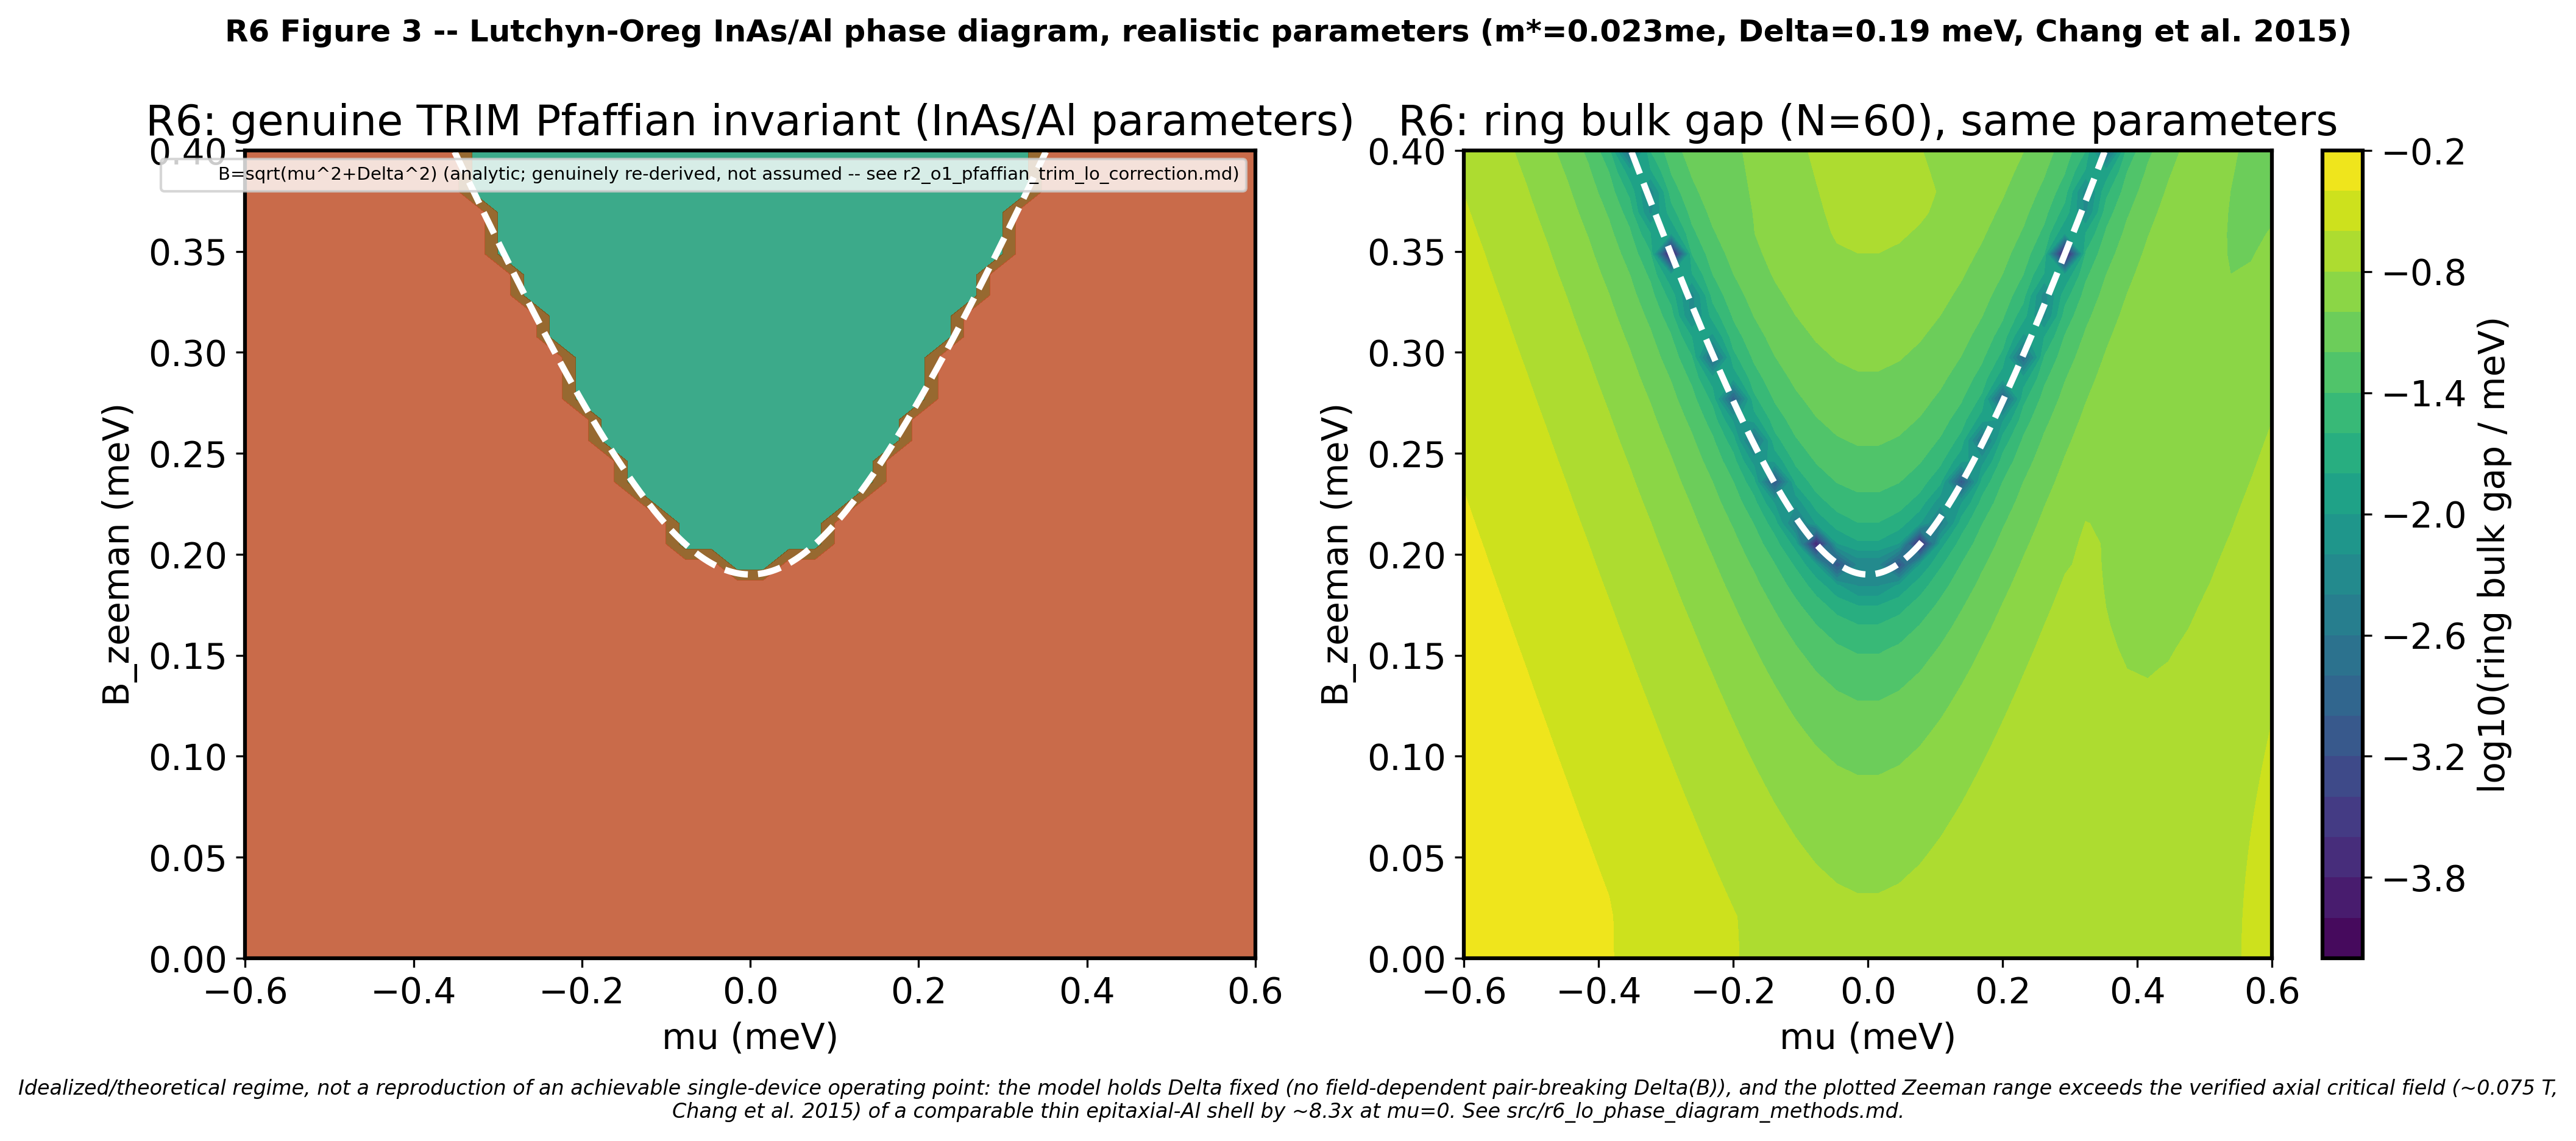
\includegraphics[width=\columnwidth]{figures/fig1_phase_diagram.png}
\caption{\textbf{The single-channel baseline: the genuine topological
invariant and the bulk gap agree with each other and with the analytic
phase boundary at every point tested.} Single-channel Lutchyn-Oreg
$(\mu,B_{\rm zeeman})$ phase diagram at realistic InAs/Al parameters:
genuine TRIM Pfaffian invariant (left) and ring bulk gap on a log scale
(right), analytic boundary $B_c=\sqrt{\mu^2+\Delta^2}$ overlaid as a
white dashed curve -- the gap visibly closes exactly where the invariant
flips sign. Idealized/theoretical regime: $\Delta$ is held fixed (no
field-dependent pair-breaking), and the plotted Zeeman range exceeds the
verified axial critical field of a comparable epitaxial-Al shell by a
factor of $\sim8$ at $\mu=0$~\cite{chang2015}. Generated by
\texttt{bdg\_r6\_lo\_phase\_diagram.py}; data in \texttt{results/lutchyn\_\allowbreak oreg\_\allowbreak phase\_\allowbreak diagram/}.}
\label{fig:phasediagram}
\end{figure}

Figure~\ref{fig:phasediagram} fixes the single-channel baseline against
which every multi-subband result below is compared: the genuine TRIM
Pfaffian invariant (left panel) and the ring's bulk gap on a log scale
(right panel), swept over the same $(\mu,B)$ grid at realistic InAs/Al
parameters, agree with each other and with the analytic boundary
$B_c=\sqrt{\mu^2+\Delta^2}$ -- the gap closes exactly where the invariant
changes sign, at every $\mu$ tested. Realistic InAs/Al devices are
estimated, from multiple independent lines of evidence, to occupy far
more than one channel: a Schr\"odinger-Poisson treatment of realistic
surface charge finds that reaching a regime of only a few occupied
subbands is ``\emph{difficult or impossible},'' with ten or more subbands
occupied under realistic gating~\cite{woods2020}, and the carrier density
directly measured by Chang \emph{et al.}~\cite{chang2015} at their
devices' operating gate voltage independently implies an occupancy of
many tens of subbands under a simple parabolic-band estimate. Two further,
independent treatments reach the same conclusion by different routes:
self-consistent Schr\"odinger-Poisson modeling of the InAs/Al interface
itself finds that band bending accumulates charge and populates multiple
subbands even before any top gate is applied~\cite{mikkelsen2018hybridization},
and a unified treatment of the orbital magnetic field, proximity pairing,
and gate electrostatics on equal footing likewise finds the low-occupancy,
few-subband regime to be a narrow, gate-sensitive operating window rather
than the device's default state~\cite{winkler2019unified}. Single-channel
operation is therefore an idealization of the device -- of the same
character as the fixed-$\Delta$ idealization already carried through
every field sweep in this paper -- not a description of it.

\begin{figure}[t]
\centering
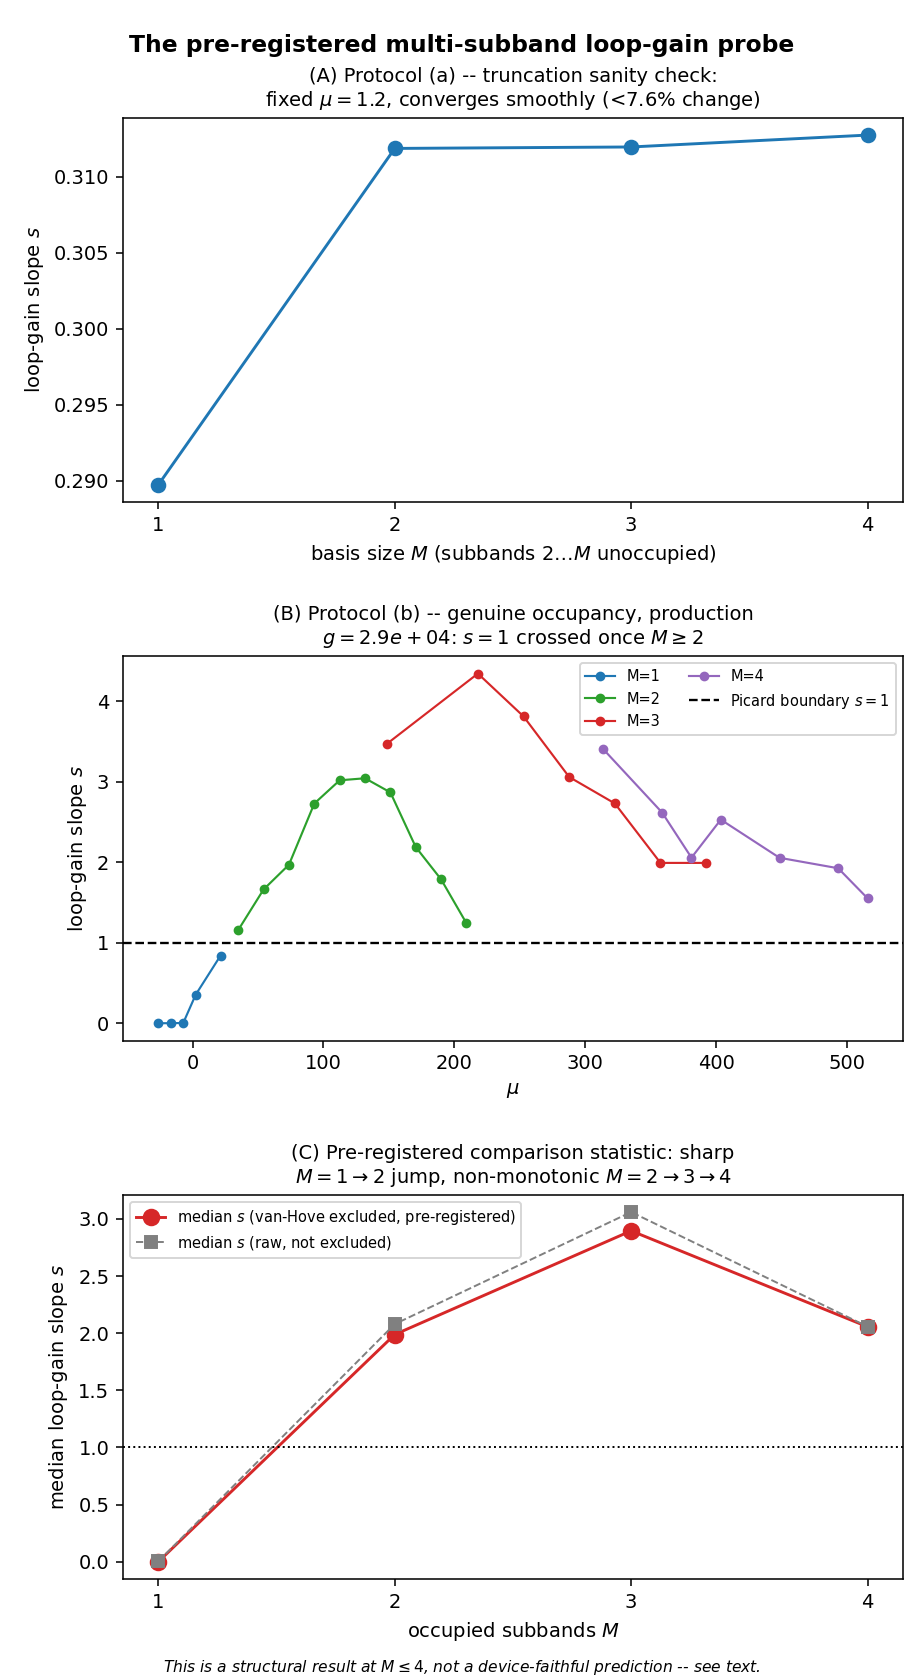
\includegraphics[width=0.82\columnwidth]{figures/fig6_multisubband_summary.png}
\caption{\textbf{Occupying a second subband crosses the Picard stability
threshold at the production electromagnetic coupling.} The pre-registered
multi-subband loop-gain probe. (A) Truncation convergence at fixed
occupancy (a construction sanity check, not the physics answer): $s$
converges smoothly with basis size, with no discontinuity. (B) The
genuine-occupancy sweep, $s(\mu;M)$ at production coupling
$g=2.9\times10^4$: the stability boundary $s=1$ (dashed line) is crossed
once $M\geq2$, and stays crossed across essentially the entire window
probed at $M=2$--$4$. (C) The pre-registered comparison statistic (median
$s$ over the surviving, van-Hove-excluded window): a sharp $M=1\to2$
jump, then a non-monotonic $M=2\to3\to4$ trend -- rising, then declining,
not settling into a clean law. \emph{This is a structural result at
$M\leq4$, not a device-faithful prediction} -- see text, and see
Fig.~\ref{fig:multisubband56} for the $M=5,6$ extension, which shows the
non-monotonicity continuing more dramatically still. Generated by
\texttt{scripts/\allowbreak redraw\_\allowbreak paper\_\allowbreak fig6.\allowbreak py} from
\texttt{results/\allowbreak multisubband/\allowbreak r9\_\allowbreak multisubband\_\allowbreak sweep\_\allowbreak data.\allowbreak json}, which
\texttt{bdg\_\allowbreak r9\_\allowbreak multisubband\_\allowbreak sweep.\allowbreak py} writes.}
\label{fig:multisubband}
\end{figure}

\begin{figure}[H]
\centering
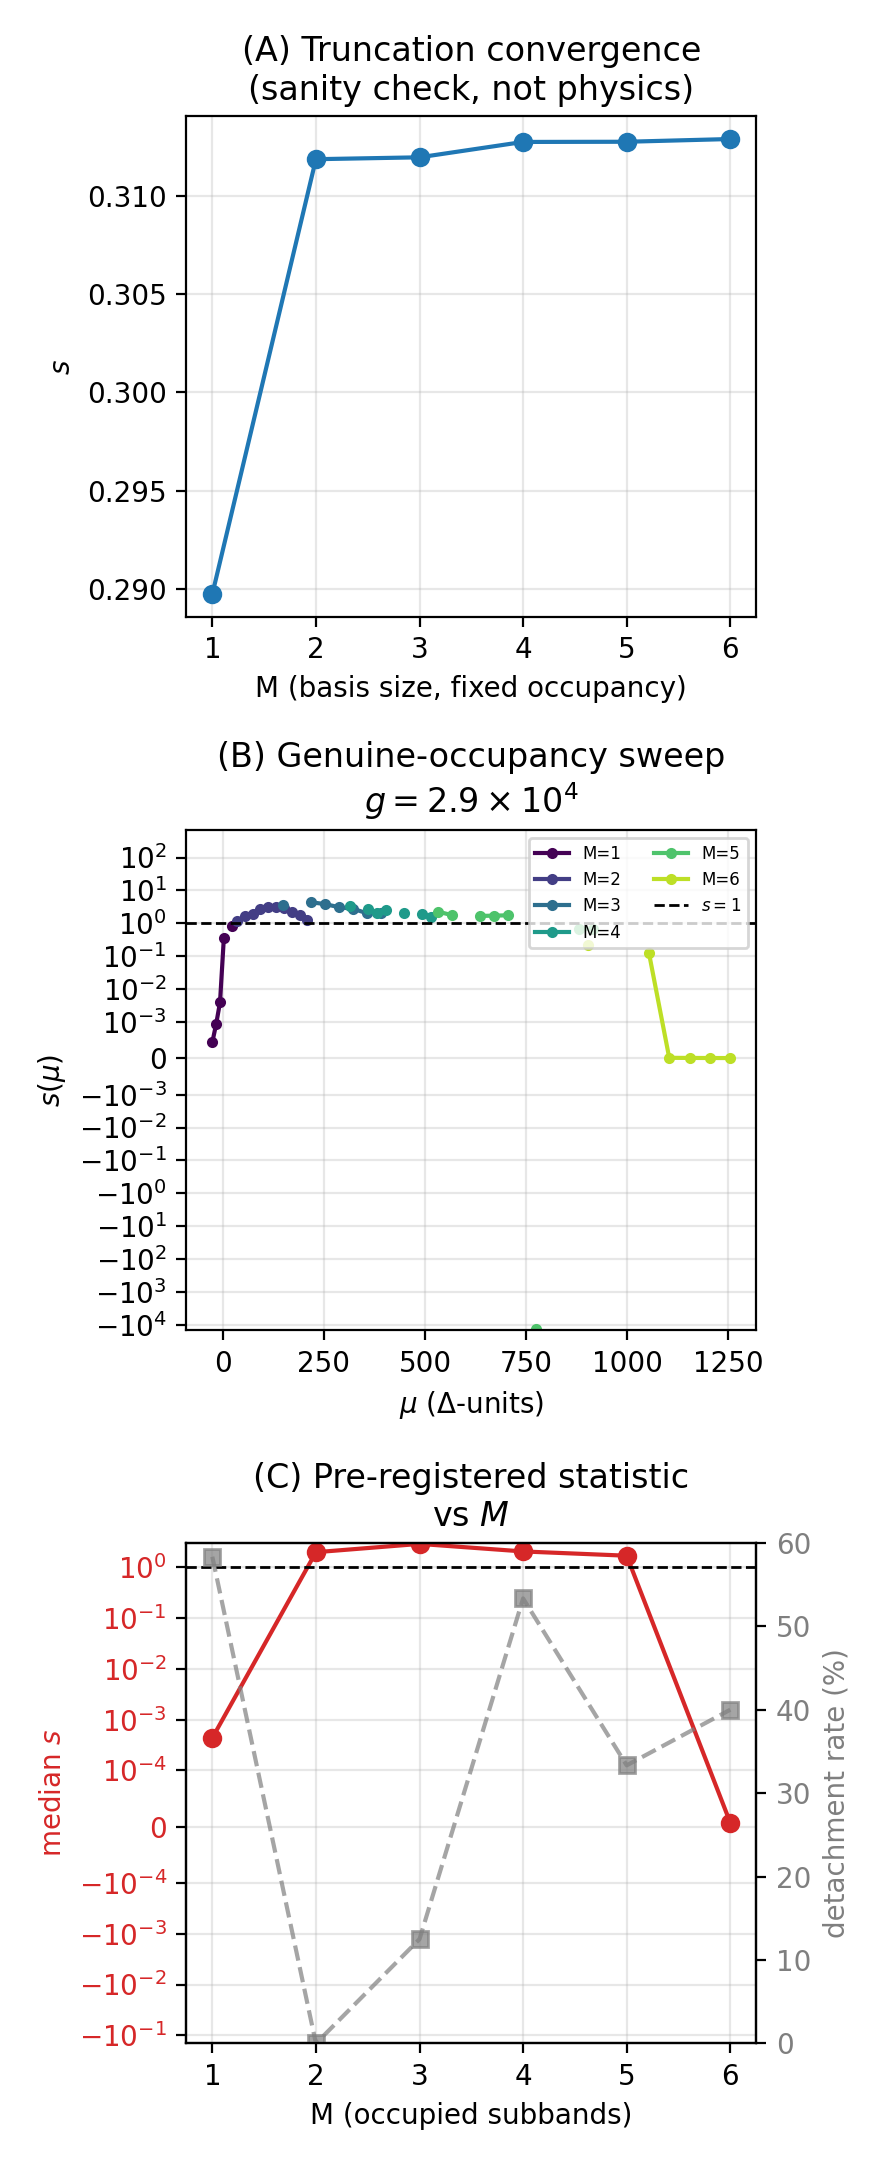
\includegraphics[width=0.82\columnwidth]{figures/fig7_multisubband_M1to6_extension.png}
\caption{\textbf{The $M\geq2$ instability is not monotonic: the
loop-gain magnitude collapses at $M=6$ while the detachment rate stays
high -- existence, not magnitude, is the operative diagnostic.} The
$M=5,6$ extension of the pre-registered multi-subband loop-gain probe
(cf.\ Fig.~\ref{fig:multisubband}), using the identical protocol
throughout -- same closed-form window, van Hove exclusion radius, and
median statistic, pre-registered before any $M=5,6$ value was computed.
(A) Truncation convergence at fixed occupancy, extended through $M=6$:
still smooth, no discontinuity, confirming the machinery itself remains
correct at higher $M$. (B) The genuine-occupancy sweep $s(\mu;M)$ at
production coupling, $M=1$--$6$ (colored by $M$, dashed line at the
Picard threshold $s=1$); gaps in a curve are genuine detachments (no
self-consistent root exists at that $\mu$), not omitted data -- note the
$M=5$ curve's excursion to $s\approx-1.4\times10^4$ near its own
detachment, and the $M=6$ curve's smooth decay to $s\approx0$ far from
its threshold. (C) The pre-registered median statistic (red, left axis)
alongside the detachment rate (gray dashed, right axis) at each $M$: the
$M=6$ collapse in the median \emph{coincides with}, rather than
\emph{replaces}, a persistently high detachment rate -- the median
statistic is not evidence of restored stability. Generated by
\texttt{bdg\_r9\_multisubband\_plot\_M6.py} from
\texttt{bdg\_r9\_multisubband\_sweep\_M56.py}'s output; data in
\texttt{results/multisubband/}.}
\label{fig:multisubband56}
\end{figure}

Using the pre-registered protocol of \S\ref{sec:model}D, the loop-gain
slope $s$ at $\mu=1.2$ (fixed occupancy, a construction sanity check
rather than the physics answer) converges smoothly with basis size $M$
from $0.290$ ($M=1$) to $0.313$ ($M=6$), an $8.0\%$ total change with no
discontinuity across the entire range tested (extended to $M=6$ at
negligible extra cost, $\sim3.5$ min for both new points combined), and
its $M=1$ value independently reproduces the single-channel result of
\S\ref{subsec:impedance} to three significant figures -- a strong
cross-check that the multi-subband machinery is physically correct, not
merely internally consistent (Fig.~\ref{fig:multisubband}A). The genuine
test -- re-tuning $\mu$ upward with $M$ so that each new subband is
actually occupied, at fixed production coupling $g=2.9\times10^4$ --
gives a qualitatively different result (Fig.~\ref{fig:multisubband}B,C).
Using only the pre-registered, van-Hove-excluded median statistic, the
loop gain is $0.0004$ ($M=1$), $1.99$ ($M=2$), $2.90$ ($M=3$), $2.06$
($M=4$), $1.70$ ($M=5$), and $7.0\times10^{-6}$ ($M=6$)
(Table~\ref{tab:m56extension}; Fig.~\ref{fig:multisubband56} extends
panels B and C of Fig.~\ref{fig:multisubband} to $M=5,6$, using the
identical closed-form window, van Hove exclusion radius, and median
statistic, pre-registered in a separate commit before any $M=5,6$ value
was computed -- the same discipline as the original $M\leq4$ protocol).
At $M=1$, $s$ stays safely sub-critical everywhere a solution is found
(maximum $0.84$); at $M=2$, $M=3$, and $M=4$, $s$ exceeds the
Picard-stability boundary $s=1$ at \emph{every individual finite point
probed}, not merely in the median. This is a qualitatively different,
and more severe, kind of finding than a percentage change in a boundary
location: merely occupying a second transverse channel, with no change
whatsoever to the electromagnetic coupling $g$, moves the wire from
``safely sub-critical at production coupling'' to ``the static
self-consistency map has Picard-repelling roots at production coupling,
across the entire window probed.''

This pattern does not continue smoothly to $M=5,6$. At $M=5$,
three-quarters of the finite points probed ($6$ of $8$) still exceed
$s=1$; the two that do not sit at the window's far edge, well above the
newly-occupied channel's own threshold. At $M=6$ the reversal is
complete: \emph{none} of the six finite points probed exceeds $s=1$, and
the median collapses four orders of magnitude below even the $M=1$
value. Taken alone, this could be misread as the instability healing
itself at $M=6$. Two features of the same dataset argue against that
reading. First, the decay is not new physics specific to $M=6$: it is
already visible at $M=5$'s window edge, and its location matches exactly
what the physical-origin argument below predicts -- the van
Hove-enhanced response is concentrated near the newly-crossed threshold
and falls off deeper into the occupied channel, and because the
pre-registered window widens linearly with $M$ ($\Delta E_{\rm
sb}(M)=\varepsilon_1(2M+1)$, \S\ref{sec:model}D) while the enhanced
region does not, an ever-larger fraction of each window's points sample
this decayed, off-threshold regime as $M$ grows. The median statistic at
$M=6$ is therefore not measuring a smaller instability so much as it is
increasingly dominated by the part of the window where the instability
was never expected to be largest. Second, and more fundamentally,
$M=6$'s own dataset does not show a return to a well-behaved static
boundary: the detachment rate (points where no self-consistent solution
exists at all, defined precisely in \S\ref{subsec:existence}) is $58\%$,
$0\%$, $12.5\%$, $53\%$, $33\%$, and $40\%$ of probed points at
$M=1$--$6$ respectively -- $M=6$'s $40\%$ sits squarely inside that
range, not a return to $M=2$'s clean $0\%$. A collapsing median loop-gain
alongside a persistently high detachment rate is not evidence that the
self-consistency map has become well-behaved at $M=6$; it is evidence
that the cheap loop-gain proxy itself becomes an unreliable summary once
detachments and off-threshold sampling dominate the window it is
evaluated over -- reinforcing, rather than undermining,
\S\ref{subsec:existence}'s conclusion that the proxy's verdict cannot
substitute for a full self-consistent boundary calculation. The full
calculation itself remains out of reach at $M=5,6$ for the same cost
reason established at $M=2$--$3$ (\S\ref{subsec:existence}): the $M=6$
proxy sweep already required $\sim4.1$ hours at $\sim30$ eigensolves per
point, against an estimated $\sim2000$ eigensolves per point for the
full boundary bisection.

\begin{table}[t]
\caption{The pre-registered loop-gain statistic and detachment rate at
every $M$ tested, $M=1$--$6$ ($N=80$, $g_{\rm production}=2.9\times10^4$).
$M\leq4$ reproduces the original sweep exactly; $M=5,6$ is the extension
reported here, computed with the identical protocol. ``finite/total''
counts the raw points where a self-consistent root was found at all
(the complement is the detachment rate); ``finite $>1$'' is the fraction
of those roots exceeding the Picard threshold $s=1$.}
\label{tab:m56extension}
\begin{ruledtabular}
\begin{tabular}{cccccc}
$M$ & points & finite/total & detach.\ \% & median $s$ & finite $>1$ \\
\hline
1 & 12 & 5/12  & 58\%   & $4\times10^{-4}$   & $0\%$   \\
2 & 10 & 10/10 & 0\%    & $1.99$             & $100\%$ \\
3 & 8  & 7/8   & 12.5\% & $2.90$             & $100\%$ \\
4 & 15 & 7/15  & 53\%   & $2.06$             & $100\%$ \\
5 & 12 & 8/12  & 33\%   & $1.70$             & $75\%$  \\
6 & 10 & 6/10  & 40\%   & $7.0\times10^{-6}$ & $0\%$   \\
\end{tabular}
\end{ruledtabular}
\end{table}

Why would occupying a second subband increase the loop gain at all,
rather than simply adding a second, independent contribution to the
current? Three considerations, taken together, offer a physically
grounded candidate answer; we do not claim any one of them individually
as a demonstrated mechanism. First, the inter-subband Rashba coupling of
\S\ref{sec:model}D is not an optional refinement but a physically
mandatory term~\cite{lim2012}, so occupying a second channel does not add
a second, additive current pathway -- it reorganizes the current-response
structure of the whole coupled system, by the same mechanism through
which Lim \emph{et al.}\ find inter-subband mixing simultaneously
hybridizing the Majorana pairs and closing the effective gap. Because $s$
is a response function governed by the low-energy spectrum, a mechanism
that closes the gap preferentially near a lobe crossing is also a
mechanism that enhances $s$ there: a smaller excitation gap admits a
larger induced-current response to a fixed external phase perturbation.
Second, every newly occupied subband threshold is a one-dimensional van
Hove singularity in the density of states, $\rho(E)\propto(E-\varepsilon_n)^{-1/2}$
(\S\ref{sec:model}D); the pre-registered protocol requires channel $M$ to
be genuinely occupied, so the sampled $\mu$-window sits close to that
singularity by construction at every $M\geq2$, even after the reported
statistic's own exclusion radius removes its immediate neighborhood --
the excluded-window median is therefore a conservative reading of the
enhancement, not an upper bound on it. Third, no inter-channel coupling
is even required for $s$ to grow with $M$: because $s$ is the derivative
of a current-sourced self-field with respect to the phase that sources
it, an approximately additive, channel-by-channel contribution to the
ring current is already sufficient on its own to move $s$ toward and
eventually through the Picard threshold as more channels are added.
Disentangling how much of the measured growth is carried by additive
current summation versus van~Hove enhancement versus genuine
inter-subband gap-closing reorganization would require directly
characterizing the current-phase relation itself -- a quantity measured
directly in InAs Josephson junctions in the few-mode
regime~\cite{hart2019currentphase} but not yet computed in this
self-consistency loop, which \S\ref{sec:discussion}B already lists as
beyond the scope of this work.

The trend with $M$ is not strictly monotonic: $s$ rises sharply from
$M=1$ to $M=3$ and then declines from $M=3$ to $M=4$ (a $\sim29\%$ drop).
This non-monotonicity is reported as measured, not smoothed into a clean
law, because establishing it required its own correction: the original $M=4$
statistic ($3.40$) rested on a single surviving point out of a sparse
five-point pre-registered grid, and re-running that one chain at three
times the point density (within the identical, unchanged pre-registered
window) revealed the same rise-then-decline shape already visible at
$M=2,3$ and reduced the reported value to $2.06$. A parallel post-hoc
investigation (holding the pre-registered statistic itself fixed
throughout) established that essentially every apparent detachment in
this dataset is not a genuine absence of a root but a root that
\emph{is} found and then rejected by the same discontinuity-rejection
criterion this project had already established, independently, as
physical rather than numerical in the single-channel case
(\S\ref{subsec:bifurcation}) -- and that this sawtooth structure, once probed
at matching resolution, is present at every $M$ tested, not only where it
happened to dominate the coarse pre-registered grid. What distinguishes
the more severely affected subband counts is not how much of this
structure is present, but how often the map fails to leave behind even
one surviving, accepted root once the structure is present. We regard
this as a genuine, reportable, unresolved feature of the multi-subband
self-consistency map's internal structure, not as either a bug or a
device-faithful prediction: this is a study truncated at $M\leq6$
subbands, far below the $10$--$26$ or more subbands realistic devices are
estimated to occupy~\cite{woods2020}, and adding even one subband can
flip the topological invariant's parity~\cite{lim2012}, so this trend --
including its own non-monotonicity -- must not be extrapolated smoothly
into the many-subband regime. The $M=5,6$ extension above is a direct
illustration of exactly this warning: had the study stopped at $M=4$, as
originally scoped, a reader could reasonably have inferred a clean,
monotonically-worsening instability with occupied-channel count; two
further, cheaply obtained data points show instead that neither the
loop-gain magnitude nor the detachment rate settles into a simple trend
anywhere in the range tested.

\FloatBarrier
\subsection{Beyond the proxy: existence, not just magnitude, of the boundary becomes fragile at $M=2$}
\label{subsec:existence}

\begin{table}[t]
\caption{The full self-consistent boundary calculation at one
representative $M=2$ operating point ($\mu=131.762$, production coupling
$g=2.9\times10^4$), as a function of system size $N$. A \emph{genuine},
Anderson-mixing-confirmed root and boundary was found at $N=80$; both
neighboring system sizes tested return a robust no-solution
(\texttt{genuine\_dead\_zone}) result across every one of five
independently jittered search paths -- the opposite $N$-dependence
pattern from the single-channel case, where dead-zones shrink and vanish
as $N$ grows. The $N=80$ shift is not quoted as a headline value; see
text.}
\label{tab:m2existence}
\begin{ruledtabular}
\begin{tabular}{ccc}
$N$ & outcome & $\Delta B_c/B_c$ \\
\hline
60  & dead zone (5/5 fail) & --- \\
80  & solution found & $-0.82\%$\footnote{Non-continuum-limit value; explicitly not a headline number---see text.} \\
120 & dead zone (5/5 fail) & --- \\
\end{tabular}
\end{ruledtabular}
\end{table}

The loop-gain slope is a cheap proxy: it asks whether a root of the
self-consistency equation at one fixed field is Picard-stable, not
whether a genuine, bisected self-consistent \emph{boundary} -- the
quantity every single-channel headline number in this paper actually
reports -- exists at all near a subband threshold. A full self-consistent
boundary calculation at $M=2$, at the same computational cost per point
as the single-channel case, is intractable as a systematic sweep (an
estimated $35$ hours at $M=3$ alone, scaling from the measured
single-channel cost), so we perform it at exactly one representative
operating point: $\mu=131.762$, near the peak of the $M=2$ loop-gain
curve above, at production coupling. Every new piece of machinery this
calculation needed -- the $M$-subband Pfaffian invariant, the $M$-subband
self-consistent boundary solver, and the uniform-current-texture
reduction the scalar loop-gain map itself depends on -- is gated
bit-for-bit against its single-channel counterpart before any $M=2$
number is trusted, and all gates pass exactly.

At $N=80$, the loop-gain proxy's root is confirmed genuine and
dynamically meaningful by the identical Anderson-mixing seed-independence
test used in \S\ref{subsec:bifurcation}: five independent seeds converge to the
same point to within $7\times10^{-11}$, while plain Picard iteration does
not converge in $200$ iterations -- exactly the repelling-but-real
signature established there. The full boundary bisection then locates a
genuine self-consistent boundary, inside a real four-lobe Pfaffian
oscillation already present in the non-self-consistent (clean)
Hamiltonian at the same $\mu$ (the literature's predicted multi-subband
phase structure~\cite{potterlee2010,potterlee2011,lutchyn2011,stanescu2011},
not a self-consistency artifact), with a shift of $-0.82\%$ relative to the
clean boundary for the same lobe -- roughly thirteen times the
single-channel shift at the identical production coupling
(\S\ref{subsec:bifurcation}).

This number is not the finding we report. The same finite-size check
applied to every quantitative shift in this paper, applied here for the
first time at $M=2$, does not show it shrinking toward zero, growing
toward a bulk value, or doing anything a single number could summarize:
at $N=60$ and $N=120$, \emph{every one} of five independently jittered
search paths returns a robust no-solution result across the entire
$B$-range where $N=80$ found its root (Table~\ref{tab:m2existence}) --
the opposite pattern from every single-channel finite-size scan in this
paper, where dead-zones shrink and disappear as $N$ grows. The $N=80$
solution is not the lucky survivor of an unstable search: each
neighboring failure is independently confirmed by all five retry paths,
which if anything makes the $N=80$ success look like the outlier in the
sequence, not the two failures around it. We therefore report this as a
genuinely mixed outcome, not a clean confirmation or a clean null: a
real, dynamically confirmed self-consistent boundary shift \emph{was}
measured at one system size, but its existence -- not merely its
magnitude -- is fragile against finite-size variation in a way
qualitatively more severe than anything in the single-channel study,
where a well-defined static boundary was always at least locatable away
from a narrow, genuinely gap-closing-related, $N$-shrinking dead-zone.
The correct, defensible statement is that at a representative $M=2$
operating point where the loop-gain proxy already signals Picard
instability, the full calculation shows that whether a static,
self-consistent topological boundary description exists \emph{at all} is
itself unstable to how finely the wire is discretized -- a strictly
stronger and more concerning statement than any specific percentage
shift, and one the cheap loop-gain proxy alone could not have revealed,
since it only ever evaluates a root at one fixed field and never asks
whether a bisected boundary exists.

\FloatBarrier
\section{Discussion}
\label{sec:discussion}

\subsection{The multi-subband caveat, restated as this paper's operative conclusion}

The single-channel result of \S\ref{subsec:bifurcation},~\ref{subsec:robustness} is a genuine, heavily
cross-validated null across finite size, circuit inductance, realistic
operating temperature, and the lower half of a literature-grounded
disorder range. It is not stated as the paper's headline, because
\S\ref{subsec:proxy},~\ref{subsec:existence} show directly that this null does
not extend past the single-conducting-channel idealization, and
independent literature estimates place realistic InAs/Al devices at ten
or more occupied subbands~\cite{woods2020,chang2015} -- an idealization
gap of the same character, and comparable seriousness, as the fixed-$\Delta$
idealization already carried through every field sweep in this paper.
The two multi-subband findings compound rather than merely add: the
loop-gain proxy shows the production coupling is already
\emph{super}-critical at every finite point tested for $M=2$, $3$, and
$4$; and the one full calculation performed shows that even the more
basic question -- does a well-defined static description exist at all --
can fail to have a stable answer as a function of lattice discretization
at exactly this occupancy. Extending the proxy sweep to $M=5,6$
(\S\ref{subsec:proxy}) complicates the magnitude axis specifically without
resolving the existence axis: the median loop gain does not continue
rising or even staying super-critical past $M=5$, but the detachment
rate -- the more fundamental of the two diagnostics, since it asks
whether a static description exists at all rather than how unstable it
is where one does -- stays high and non-monotonic at every $M$ tested,
including $M=6$. Neither finding is a device-faithful prediction (both
are structural results at $M\leq6$, against a real device's estimated
$10$--$26$ or more occupied subbands, and a subband can flip the
topological invariant's parity~\cite{lim2012}), but together they mean the
single-channel null result's applicability to a real device is not merely
an open question -- it is a \emph{specifically and concretely troubled}
one, in a way our data can characterize but not resolve.

\subsection{Limitations}

Several idealizations are carried through every result in this paper and
are not resolved here. First, the pairing potential $\Delta$ is held
fixed and does not include field-dependent pair-breaking; a more complete
model would suppress $\Delta(B)$ toward zero as $B$ approaches a real
device's critical field, likely rounding off or eliminating the sharp
transitions plotted at the largest fields shown. Because the analytic
boundary used throughout this paper, $B_c=\sqrt{\mu^2+\Delta^2}$, depends
explicitly on $\Delta$, a genuine $\Delta(B)$ would mean the transition
boundary itself is no longer a fixed target but one that depends on the
field history used to reach it -- a qualitative feature the present
fixed-$\Delta$ model cannot capture by construction. It is plausible,
though not established by anything computed here, that this could affect
not only where the boundary sits but also the self-consistency loop's own
dynamical bifurcation structure: since $g_{\rm crit}$
(\S\ref{subsec:bifurcation}) is set by the loop-gain slope of a
self-consistency map that itself depends on the underlying spectrum, a
pairing potential that locally weakens near the transition could in
principle shift where that slope crosses unity. We state this as informed
speculation about the likely qualitative direction of the effect, not a
quantitative prediction; computing it would require implementing a
genuine $\Delta(B)$ model, which is explicit future work
(\S\ref{sec:discussion}C). Second, the literature
plausibility range for the electromagnetic coupling $g$ spans regimes on
both sides of the dynamical bifurcation identified in
\S\ref{subsec:bifurcation}; the argument was never specific enough to establish
which side a given real device sits on, and what physically happens
above $g_{\rm crit}$ -- whether a real device simply never reaches that
regime, or whether the feedback becomes genuinely dynamical (e.g.\ a
current/self-field limit cycle) rather than settling to any static
picture -- is not resolved by this work. Third, two specific mechanisms
in the multi-subband dataset remain open: why the self-consistency map's
candidate-crossing rejection rate differs so sharply between subband
counts that show the same or greater raw sawtooth structure, and whether
the one $N=80$ window found for the $M=2$ full boundary calculation is a
genuine (if fragile) physical solution or a lattice-commensurability
artifact of that specific system size. Both would require direct
characterization of the current-phase relation itself, not just its
zero-crossings, which is beyond the scope of this work.

\subsection{Future work}

The most direct extensions are: a genuine field-dependent pairing
suppression $\Delta(B)$; a derivation of the electromagnetic coupling $g$
from a specific, named circuit design rather than a plausibility range;
and, most importantly given \S\ref{sec:discussion}A, any tractable route
toward the full self-consistent electromagnetic feedback calculation at
occupancies closer to a real device's estimated $10$--$26$ subbands,
which is intractable with the present per-point cost and would require
either substantially more compute or a genuinely cheaper self-consistent
solver than the one used throughout this paper.

A natural experimental question is what signature, if any, could
distinguish this paper's findings from a null hypothesis in a real
device. Three directions seem most plausible given what is established
here, listed in order of how directly each targets the paper's own
operative conclusion (\S\ref{sec:discussion}A).

First, and most directly: since the existence-fragility result is a
statement about occupied-\emph{channel count}, and depletion gates
already tune real devices toward (though, per Sec.~\ref{subsec:proxy}, not
reliably into) a low-occupancy regime~\cite{mikkelsen2018hybridization,winkler2019unified},
a gate-voltage scan that steps the wire through successive subband
depopulations while monitoring a circuit-level observable at fixed,
production-scale coupling is a direct experimental analogue of this
paper's $s(\mu;M)$ sweep (\S\ref{subsec:proxy}). The predicted signature is
qualitative, not a specific number to match: an increase in circuit
noise, hysteresis, or measurement instability correlated with each
successive gate step that adds a conducting channel, consistent with the
Picard-repelling regime identified here, rather than a smooth, monotonic
trend. Second, the reactive-impedance diagnostic of
\S\ref{subsec:impedance} is, in principle, a directly measurable
circuit-level quantity -- by dispersive microwave readout of the kind
already used to probe parity-dependent inductance and capacitance in
related Majorana and Andreev-bound-state
circuits~\cite{ginossar2014microwave,roy2026inductance} -- but our own
finding that $Z_r$ carries essentially no topological information the
bulk gap does not (\S\ref{subsec:impedance}) is itself a direct caveat on
how informative such a measurement would be as a diagnostic of \emph{this
paper's} physics specifically, even though it is measurable in principle.
Third, fabricating devices with deliberately varied loop geometries or
lengths -- the experimental analogue of this paper's own computational
circuit-inductance scan (\S\ref{subsec:bifurcation}) -- could probe
whether real devices show any of the finite-size or dynamical-stability
signatures identified here, such as the dead-zone regime opening at
shorter loop lengths. We state these as the most plausible directions
given what this paper establishes, not as experiments we expect would
confirm or refute any specific claim made here.

\section{Conclusion}

We have built and validated a computational framework that closes the
loop between a Majorana nanowire's self-generated electromagnetic field
and its own topological phase boundary, using a genuine, threshold-free
topological invariant throughout. In the single-conducting-channel limit
this feedback does not move the bulk topological boundary at any
dynamically accessible coupling strength, and this null result is robust
under finite-size scaling, circuit inductance, realistic operating
temperature, and the lower half of a literature-grounded disorder range.
Two methodological lessons -- that a conventional threshold detector is
not a reliable proxy for the topological invariant, and that a
self-consistency loop's mathematical roots must be checked for dynamical
attractiveness separately from their existence -- recur throughout this
result and, we believe, generalize beyond this specific calculation.
Extending the calculation to a second occupied transverse subband
overturns the null result: a validated loop-gain diagnostic crosses the
stability threshold at production coupling once two or more subbands are
occupied, and a full self-consistent calculation at one representative
two-subband point shows that the very existence of a static topological
boundary description becomes fragile to the lattice discretization used
to compute it. Because realistic InAs/Al devices are estimated to occupy
far more than two subbands, this existence-fragility result -- not the
single-channel null in isolation -- is the finding that should inform how
electromagnetic feedback is treated in realistic Majorana nanowire
devices, and we regard resolving it as the natural next step for this
line of work.

\begin{acknowledgments}
The author thanks Jagadis Prasad Nayak (NIT Rourkela) for reviewing the
manuscript and for assistance in editing the draft, and the open-source
scientific Python ecosystem (\texttt{NumPy}, \texttt{SciPy},
\texttt{pfapack}, \texttt{Matplotlib}) that this work's computational
framework is built on.

The author used AI assistants (Anthropic's Claude, including Claude
Code) for software development, analysis scripting, and drafting. All
results were checked by the author using the validation gates described
in this paper, and the author takes full responsibility for the content.
\end{acknowledgments}

\appendix

\section{The reduced-order BdG eigensolver and its actual scope}
\label{app:eigensolver}

The computational framework includes a particle-hole-symmetric rank-2
subspace update for the near-zero-mode sector of the BdG Hamiltonian,
intended to accelerate the repeated diagonalizations performed along a
parameter path (steps in $\mu$, $B$, $\Delta$, or the self-field Peierls
phase $\phi$). For a rank-2 perturbation confined to the near-zero-mode
subspace, the update reproduces the full-diagonalization near-zero
eigenvalues to $9.4\times10^{-6}$, so the technique itself is correct.

We nonetheless report a genuine limitation on its usefulness for this
project, rather than presenting it as an unqualified speedup, because that
is what the measurements show. First, the update's conservative
eigenvector-residual safety net -- which falls back to a full solve
whenever the rank-2 residual exceeds $10\lVert\delta H\rVert$ -- trips on
the self-field phase steps the self-consistency loop actually takes (the
eigenvector residual is $\approx5\times10^{-3}$ against a threshold
$\approx3.6\times10^{-3}$), so in practice it falls back to a full solve on
every probed step. Second, and more fundamentally, the ring current that
sources the self-field sums over the \emph{entire} occupied BdG spectrum,
so each self-consistency iteration requires the full set of occupied
eigenvectors; the dense diagonalization is $96$--$98\%$ of the
per-iteration cost, and a near-zero-mode subspace update cannot supply what
dominates that cost. The net effect on the flagship self-consistent loop is
therefore $\sim\!1\times$: the subspace update is a validated, correct
technique that does \emph{not} accelerate the calculation this paper's main
results depend on, reported as such rather than as a speedup that does not
apply here. (An earlier internal description of this update as
a Woodbury-type low-rank identity was corrected during this work: the
perturbations that actually arise are full-rank, so the Woodbury identity
does not apply, and the construction is more accurately described as a
subspace update.)

\section{Validation gates}
\label{app:gates}

Every physics layer added over the course of this work was gated against a
known limit -- an analytic boundary, an exactly solvable decoupled case, a
symmetry identity, or a bit-for-bit reduction to an already-validated lower
layer -- before any result computed with that layer was trusted.
Table~\ref{tab:gates} collects these gates and their measured outcomes.
Many are enforced exactly ($0.0$) or at machine precision, because they
compare two constructions that must be entrywise identical -- for example,
a disorder-aware builder at zero disorder against its clean counterpart, or
a multi-subband Hamiltonian at one subband against the single-channel one;
others are agreements to a stated tolerance against an analytic result. The
value of collecting them is not any single number but the discipline they
encode: no layer was trusted on plausibility, each gate is a falsifiable
check with a pre-stated pass criterion, and every one is reproducible from
the scripts in the public repository (\S\ref{sec:dataavail}). A gate that
reduces to a bit-for-bit identity at the known limit is preferred over an
agreement ``to $10^{-12}$'' wherever the two constructions are meant to be
literally the same object, because only the former distinguishes a correct
implementation from one that is merely close.

Two procedural points referenced from the main text are recorded here in
full. First, the Pfaffian $B_c$ detector's validation sweep
(\S\ref{sec:model}B) checked agreement against the analytic boundary
$B_c=\sqrt{\mu^2+\Delta^2}$ at $\mu=0$ and at two additional, deliberately
non-round values of $\mu$ (giving an irrational $B_c$, so agreement
cannot be a coincidence of symmetry), across ring sizes $N=20$--$160$ and
across bisection tolerances spanning four orders of magnitude; the
corresponding measured outcomes are the first three rows of
Table~\ref{tab:gates}. Second, the Newton-Krylov search for a
symmetry-broken self-consistent solution (\S\ref{sec:model}C) is seeded
with large perturbations -- up to three flux-quantum periods in
magnitude -- applied along the system's most Picard-unstable texture
modes, so that the search is deliberately biased toward finding a
non-uniform solution if one exists rather than merely probing small
perturbations around the uniform one; every tested seed nonetheless
collapses back to the uniform solution.

\onecolumngrid
\begingroup
\squeezetable
\begin{table}[H]
\caption{Validation gates enforced before any result computed with a given
layer was trusted. ``Bit-for-bit'' / $0.0$ entries compare two
constructions required to be entrywise identical at the stated limit;
tolerance entries are agreements against an analytic or independently
computed reference. All are reproducible from the public repository.}
\label{tab:gates}
\begin{ruledtabular}
\begin{tabular}{lll}
Layer & Gate (known limit or identity) & Measured result \\
\hline
Pfaffian $B_c$ detector      & known answer at $\mu=0$, $B_c=\Delta$, $N=20$--$160$      & $B_c=1.00004$; spread over $N$ $=0.0$ \\
Pfaffian $B_c$ detector      & non-round $\mu=0.7,1.3$ (irrational $B_c$), $N=20,60,120$ & error $\pm3.8\times10^{-8}$, $N$-independent \\
Pfaffian $B_c$ detector      & bisection-tolerance tracking, $N=20$ vs $80$              & error $\propto$ tol; agree to all printed digits \\
TRIM Pfaffian invariant      & genuine Pfaffian vs.\ closed form, 1600-point sweep       & 0 disagreements; identity to $1.5\times10^{-14}$ \\
Ring Biot--Savart self-field & uniform current vs.\ discrete-exact loop kernel           & $0.003\%$ \\
Ring Biot--Savart self-field & vs.\ analytic thin-wire loop inductance                   & $2.25\%$ (understood log-factor offset) \\
Self-consistency solvers     & bisection / Newton--Krylov / Anderson at one root         & agree to $5.5\times10^{-10}$ \\
Anderson mixing              & Anderson vs.\ bisection $B_c$, $N=80$, $\mu=1.2$          & agree to 6 significant figures \\
LO phase diagram             & Kramers degeneracy at $B=0$                                & $2N$ of $4N$ levels pair to $<10^{-8}$ \\
LO phase diagram             & zero-SOC gap closes off-TRIM, 6 $(\mu,B)$ points          & continuum gap $\sim10^{-3}$--$10^{-4}$ (grid-limited) \\
LO phase diagram             & analytic boundary $B=\sqrt{\mu^2+\Delta^2}$               & $-0.50$ grid steps (finite-resolution signature) \\
Multi-subband builder        & $M=1$ vs.\ single-channel $H$ and current $I$             & $\max|\Delta H|=\max|\Delta I|=0.0$ \\
Multi-subband builder        & decoupled limit vs.\ direct sum of $M$ blocks             & entrywise $0.0$ \\
Multi-subband builder        & particle-hole symmetry, $M=1$--$4$                        & $0.0$ \\
Multi-subband builder        & inter-subband selection rule (Hermitian, parity)          & exact \\
Multi-subband builder        & van Hove $\delta$ vs.\ diagonalized threshold spectrum    & closed form $10$--$21\%$ conservative \\
Multi-subband boundary solver& $M$-subband Pfaffian / $B_c$ vs.\ single channel at $M=1$ & $B_c$ difference $=0.0$ \\
Multi-subband boundary solver& uniform-current-texture reduction at $M=2$                & $\mathrm{std}/|\mathrm{mean}|=1.9\times10^{-13}$ \\
Finite-temperature layer     & all channels at $\theta\to0$ vs.\ $T=0$                   & $0.0$ (Kubo $\chi$: $8.9\times10^{-16}$) \\
Finite-temperature layer     & finite-$T$ DC gate, $\theta=0$--$0.15$                     & $2.5\times10^{-7}$--$4.8\times10^{-6}$ \\
Disorder layer               & all detectors at $W=0$ vs.\ clean                         & bit-identical ($0.0$) \\
Disorder layer               & particle-hole symmetry at $W=5\Delta$                     & $0.0$ (any realization) \\
Kubo impedance               & DC limit $\chi_{JJ}(0)$ vs.\ $d\langle J\rangle/d\phi$, 6 points & $\sim1\times10^{-4}$ \\
Parallel infrastructure      & serial vs.\ parallel, every track                         & $\mathrm{max\_abs\_diff}=0.0$ \\
\end{tabular}
\end{ruledtabular}
\end{table}
\endgroup
\twocolumngrid

\section{Correction ledger: superseded results are preserved, not overwritten}
\label{app:corrections}

Consistent with the data-availability statement (\S\ref{sec:dataavail}),
results that were later superseded by a more rigorous check are retained in
the repository -- labeled as superseded, with the correction and its
reasoning recorded alongside -- rather than deleted, so that the correction
history is auditable rather than invisible. The load-bearing instances,
each discussed at the relevant point in the main text:

\begin{enumerate}
\item \emph{The threshold-detector boundary shift} ($-5.86\%/-9.36\%$) is
kept alongside the threshold-free Pfaffian value ($-0.77\%/-0.60\%$ for the
same self-field), because the order-of-magnitude gap between them is itself
a reported result (\S\ref{subsec:threshold}).

\item \emph{The invariant-computation bug}, flagged in \S\ref{sec:model}B: an
earlier module computing the topological invariant at the two
time-reversal-invariant momenta of the Lutchyn-Oreg model built the
correct real, antisymmetric Majorana-basis matrices at each momentum but
never passed them to the Pfaffian routine, instead returning a hardcoded
closed-form expression that happened to reproduce the correct answer only
because of a parameter regime where the closed form and the genuine
Pfaffian provably agree ($|4t-\mu|$ large compared to $B,\Delta$, true
everywhere this codebase's parameters are used, but not true in general).
The discard was found by a line-by-line audit, traced to confirm it had
never propagated into any reported boundary-shift result (all of which
trace to an independent, always-genuine Pfaffian implementation), fixed to
call the real Pfaffian routine, and re-validated against the analytic
boundary with zero disagreements over a 1600-point sweep. We preserve this
level of detail here -- not because it changed any physics result in this
paper, but because it is a concrete instance of the validation discipline
-- catching, tracing, fixing, and re-validating a bug before trusting any
of its downstream numbers -- that this paper's data-availability and
reproducibility claims rest on.

\item \emph{The self-consistent shift at the initially assumed coupling}
($+0.05\%$ at $g=3\times10^5$) is kept, labeled, because it is what revealed
the dynamical bifurcation: it is a mathematically valid but
dynamically unreachable root, and preserving it makes the
existence-versus-attractiveness distinction (\S\ref{subsec:bifurcation})
concrete.

\item \emph{The disorder inductive-feedback shift} passed through two
recorded corrections -- a search-window coding bug, then a finite-size
inflation caught by an $N$-independence check -- with both superseded
versions preserved in the repository. The main text presents the final,
twice-corrected reading (\S\ref{subsec:robustness}), and the correction process
is itself part of the argument that a confident non-null claim at high
disorder does not survive.

\item \emph{The multi-subband $M=4$ loop-gain statistic} was revised from a
sparse-sampling value ($3.40$, one surviving point) to a properly-resolved
one ($2.06$) after densifying that chain within the identical pre-registered
window; the revision is reported rather than the original quietly replaced
(\S\ref{subsec:proxy}), as a worked example of the sampling risk the
pre-registration was designed to guard against.
\end{enumerate}

None of these corrections is presented as a footnote to be skimmed past:
where the correction process is methodologically instructive, it is part of
the paper's actual argument, which is that a spurious effect is dismantled
only by cross-checks each more rigorous than the last.

\bibliography{references}

\end{document}
